%\iffalse
% bewerbung.dtx generated using makedtx version 0.94b (c) Nicola Talbot
% Command line args:
%   -author "André Hilbig, mail@andrehilbig.de"
%   -codetitle "Implementation"
%   -setambles "neueBewerbung.sh=>\nopreamble\nopostamble"
%   -date "2015-07-14:14:18:49 -- Version 1.1"
%   -src "(.*)\.sty=>\1.sty"
%   -src "(.*)\.cls=>\1.cls"
%   -src "neueBewerbung.sh=>neueBewerbung.sh"
%   -src "(.*)\.inc=>\1.inc"
%   -doc "../dokumentation.tex"
%   -macrocode "neueBewerbung.sh"
%   -comment "neueBewerbung.sh"
%   -comment "config.inc=>config.inc"
%   bewerbung
% Created on 2015-07-14:14:18:49 -- Version 1.1/7/14 14:18
%\fi
%\iffalse
%<*package>
%% \CharacterTable
%%  {Upper-case    \A\B\C\D\E\F\G\H\I\J\K\L\M\N\O\P\Q\R\S\T\U\V\W\X\Y\Z
%%   Lower-case    \a\b\c\d\e\f\g\h\i\j\k\l\m\n\o\p\q\r\s\t\u\v\w\x\y\z
%%   Digits        \0\1\2\3\4\5\6\7\8\9
%%   Exclamation   \!     Double quote  \"     Hash (number) \#
%%   Dollar        \$     Percent       \%     Ampersand     \&
%%   Acute accent  \'     Left paren    \(     Right paren   \)
%%   Asterisk      \*     Plus          \+     Comma         \,
%%   Minus         \-     Point         \.     Solidus       \/
%%   Colon         \:     Semicolon     \;     Less than     \<
%%   Equals        \=     Greater than  \>     Question mark \?
%%   Commercial at \@     Left bracket  \[     Backslash     \\
%%   Right bracket \]     Circumflex    \^     Underscore    \_
%%   Grave accent  \`     Left brace    \{     Vertical bar  \|
%%   Right brace   \}     Tilde         \~}
%</package>
%\fi
% \iffalse
% Doc-Source file to use with LaTeX2e
% Copyright (C) 2015-07-14:14:18:49 -- Version 1.1 André Hilbig, mail@andrehilbig.de, all rights reserved.
% \fi
% \iffalse
%<*driver>
\documentclass[a4paper]{ltxdoc}
\usepackage[utf8]{inputenc}
\usepackage[T1]{fontenc}
\usepackage[english,ngerman]{babel}
\usepackage{xparse,xargs}
\usepackage{newfloat}
\usepackage[usenames,dvipsnames,svgnames,table]{xcolor}
\definecolor{blau}{rgb}{0,0,0.75}         
\definecolor{orange}{rgb}{0.8,0.3,0} 
\usepackage{filecontents}
\begin{filecontents}{bewerbung.bib}
	@electronic{komacv,
		author     = "Salome Södergan",
		month      = {Aug},
		year       = "2014",
		title      = "komacv",
		subtitle	 = "Typesetting a beuatiful CV with various style	options",
		url        = {http://www.ctan.org/pkg/komacv},
		urldate    = {2015-07-09},
	}

	@electronic{scrlttr2,
		author     = "Markus Kohm",
		month      = {Jul},
		year       = "2015",
		title      = "scrlttr2",
		subtitle	 = "Koma-Script ‘letter’ class",
		url        = {http://www.ctan.org/pkg/scrlttr2},
		urldate    = {2015-07-09},
	}

	@electronic{datatool,
		author     = "Nicola Talbot",
		year       = "2014",
		title      = "datatool",
		subtitle	 = "Tools to load and manipulate data",
		url        = {http://www.ctan.org/pkg/datatool},
		urldate    = {2015-07-09},
	}

	@electronic{pdfpages,
		author     = "Andreas Matthias",
		year       = "2015",
		title      = "pdfpages",
		subtitle	 = "Include PDF documents in LaTeX",
		url        = {http://www.ctan.org/pkg/pdfpages},
		urldate    = {2015-07-09},
	}
\end{filecontents}
\usepackage[%
	backend=biber,
	sortlocale=de_DE,
	style=authoryear,
	bibencoding=UTF8,
	block=space,
	autocite=inline,
	language=ngerman,
]{biblatex}
\addglobalbib{bewerbung.bib}
\renewcommand*{\mkbibnamelast}{\textsc}

\DeclareCiteCommand{\citeauthorfull}
  {%
		\boolfalse{citetracker}%
		\boolfalse{pagetracker}%
		\usebibmacro{prenote}}
  {\ifciteindex%
     {\indexnames{labelname}}
     {}%
		 \printnames[first-last]{author}}
  {\multicitedelim}
  {\usebibmacro{postnote}}


\usepackage{hyperref}
\hypersetup{%
 pdftitle = {\LaTeX-classes and -packages for typesetting nice applications and %
			tables of applications - \LaTeX-Klassen und -Pakete zum Setzen schöner %
			Bewerbungsmappen und einer Übersichtstabelle zur Dokumentation der % 
			Bewerbungsversuche}, %
 pdfsubject = {}, %
 pdfkeywords = {LaTeX,CTAN,applications,bewerbungen,cv,lebenslauf,arge,Agentur für Arbeit}, %
 pdfauthor = {Andr\'e Hilbig}, %
 colorlinks = true, %
 hypertexnames = true, %
 linkcolor=blau, %
 filecolor=orange, %
 citecolor=blau, %
 menucolor=orange, %
 urlcolor=orange, %
 breaklinks=true %
}

\usepackage{graphics,graphicx,textcomp}
\usepackage{placeins,float,caption,prettyref}
\usepackage{pdfpages,listings,xspace}
\usepackage{amssymb,multicol,pdflscape}
\usepackage[german=guillemets]{csquotes}
\newrefformat{sec}{Abschnitt\,\ref{#1}, S.\,\pageref{#1}}
\newrefformat{paket}{Paket~\ref{#1}, S.\,\pageref{#1}}
\newrefformat{klasse}{Klasse~\ref{#1}, S.\,\pageref{#1}}
\newrefformat{fig}{Abb.\,\ref{#1}}
\newrefformat{tab}{Tab.\,\ref{#1}}
\newrefformat{bsp}{Bsp.\,\ref{#1}, S.\,\pageref{#1}}
\newcommand{\refMacro}[1]{Makro \texttt{\textbackslash#1}, S.\,\pageref{#1}}
\DeclareFloatingEnvironment[name={Bsp.},
	listname={Beispielverzeichnis}, within=section]{example}
\floatstyle{ruled}
\restylefloat{example}
\NewDocumentEnvironment{beispiel}{o o m}{
 \begin{example}[ht!]
 \centering
 \vspace{0.2cm}
 \IfNoValueTF{#2}{
 	\caption{#3}
 }{
 	\caption[#2]{#3}
 }
 }{
	 \IfNoValueTF{#1}{
	 	\label{\theexample}
	 }{
	 	\label{#1}
	 }
 \vspace{0.2cm}
 \end{example}
 }
\DisableCrossrefs
\makeatletter
\makeatother
\lstset{  %
  language=[LaTeX]TeX,                 
  basicstyle=\small,            
  numbers=left,                    
  numberstyle=\footnotesize,           
  stepnumber=1,                    
  numbersep=5pt,                   
  backgroundcolor=\color{Peach!30!white},       
  showspaces=false,                
  showstringspaces=false,          
  showtabs=false,                  
  frame=single,
  tabsize=2,                       
  resetmargins=true,
  captionpos=b,                    
  title={},  
	caption={},	
  breaklines=true,
  breakautoindent=true,
  prebreak=\mbox{ $\curvearrowright$},
  postbreak=\mbox{$\rightsquigarrow$ },
  linewidth=\columnwidth,
  breakatwhitespace=true,         
  numberstyle=\tiny\color{gray},         
  keywordstyle=\color{OliveGreen}\textbf,           
  commentstyle=\color{gray}\itshape,        
  stringstyle=\color{mauve},          
  morekeywords={
		minisec, subsection, glqq, grqq, euro, Name, Vorname, Street,
		Plz, Stadt, MeinBeruf, EMail, Tel, Mobile, Sta, GebDatum, ID,
		Anhang, includepdf, includepdfmerge, cventry, cvlistitem,
		cvlanguage, definecolor, maketitle, makePerson, cp, ln, mkdir,
		todayOrt, todayDatum,	
  },
	literate=%
	{Ö}{{\"O}}1
	{Ä}{{\"A}}1
	{Ü}{{\"U}}1
	{ß}{\ss}2
	{ü}{{\"u}}1
	{ä}{{\"a}}1
	{ö}{{\"o}}1
	{»}{{\frqq}}4
	{«}{{\flqq}}4	
	{~}{$\sim$}1	
}

\xspaceaddexceptions{\guillemotright,\guillemotleft}

\CheckSum{2158}


\begin{document}
\DocInput{bewerbung.dtx}
\end{document}
%</driver>
%\fi
%		\title{\LaTeX-classes and -packages for typesetting nice applications and 
%			tables of applications\newline\ \newline
%			\LaTeX-Klassen und -Pakete zum Setzen schöner Bewerbungsmappen und einer
%	 Übersichtstabelle zur Dokumentation der Bewerbungsversuche}
%		 \author{Andr\'e Hilbig \\ \texttt{mail@andrehilbig.de} \\
%			 \url{http://www.andrehilbig.de/index.cgi/Publications/Bewerbung}}
%    \date{2015-07-14}
%    \maketitle
%    \begin{abstract}
%		 \foreignlanguage{english}{
%			This project has the aim to provide packages and classes for
%			typesetting an application with titlepage, letter, cv and
%			additional documents in just one document. Also there is a class
%			for printing a table with the latest applications that can be
%			shown to the german authorities. The data of the applications can
%			be edited in a simple csv file.
%		 }
%
%			Dieses Projekt hat das Ziel, Pakete und Klassen zum Setzen von
%			Bewerbungsmappen mit Titelseite, Brief, Lebenslauf und
%			zusätzlichen Dokumenten bereitzustellen. Außerdem gibt es eine
%			Klasse zum Setzen einer Tabelle mit den aktuellen
%			Bewerbungsversuchen, die der Agentur für Arbeit vorgelegt werden kann. Die
%			Daten der Bewerbungsversuche werden in einer simplen csv-Datei
%			verwaltet.
%		\end{abstract}
%\begin{multicols}{2}
% \tableofcontents
%\end{multicols}
%\vrule
%\begin{multicols}{2}
% \listofexample
%\end{multicols}
%	\clearpage
%	\begingroup
%	\selectlanguage{english}
%		\section{Introduction}
%			There are a lot of great projects for writing documents of an application in \LaTeX. 	But they
%			all got two problems you will have to find a workaround for. A normal application has a
%			titlepage, a letter, a cv and some additional documents like your diploma. There is a package
%			or class in \LaTeX\ for every part -- but in the end your application is split up in at least
%			three documents you'll have to merge. Also you'll have to put the data of yourself and the
%			company you're writing to in every document in a different way.
%
%			It's a little bit complicated to merge the functionality of all the different projects into one
%			document on \TeX-level, because you can not load different classes at one time. So I thought
%			of rewriting some of the packages. Mainly I want to thank \citeauthorfull{komacv} for his great
%			work. I simply copied his class and packages and rewrote the class to use it as a package. So
%			all the credit for the cv belongs to him.
%
%			If you loose your job in germany, you'll have to report to the authorities every application you
%			wrote to get the small charity. Otherwise the charity gets smaller. I wanted to have a
%			document that \enquote{knows} all your latest applications and throws out a table for that
%			issue. Of course that is a job for the great \citetitle{datatool} project of
%			\citeauthorfull{datatool}.
%
%			Last but not least there is the great \citetitle{scrlttr2} class for writing letters by
%			\citeauthorfull{scrlttr2}. I use it to print the letter within the document and added the
%			possibility to show a titlepage.
%
%			\subsection{Thanks}
%			Of course without the \verb|CTAN|-project none of this could have happened.
%
%			Special thanks goes to these three people for their awesome work:
%			\begin{itemize}
%				\item \citeauthorfull{scrlttr2} \autocite{scrlttr2},
%				\item \citeauthorfull{komacv} \autocite{komacv} and
%				\item \citeauthorfull{datatool} \autocite{datatool}.
%			\end{itemize}
%
%			\subsection{Hint}
%			This documentation is mainly written in german, because the package itself provides only
%			german macros. Aside from that it was designed to get applications and documentation for the
%			german authorities working together. Maybe the work could be usefull for non german too. Then
%			someone should write a wrapper for my macros -- in fact I did not touch so much of the
%			koma-internals of \verb|scrlttr2| or \verb|komacv|, perhaps it is not that bigger work.
%
%			I think the authorities in Germany demand very much work of a person potentially not
%			responsible for her/his situation. You get only a very small charity. So you have to write a
%			huge amount of applications -- even to jobs you and the companies don't care about you applying
%			for. And of course you can not be trusted to really write applications like hell.  Because of
%			that you'll have to show a documentation of all your applications to get your money.  I thought
%			we'd need a \LaTeX-package to automate this stuff and so I made it.
%	\endgroup
%	\selectlanguage{ngerman}
%
%		\section{Änderungen}
%			\begin{description}
%				\item[v1.0] Veröffentlichung
%				\item[v1.1]
%					\begin{itemize}
%						\item Leerzeichen in Anrede hinzugefügt
%						\item Kodierungs- und Spracheinstellungen aus der Klasse entfernt
%						\item Leerzeichenproblematiken entfernt
%						\item Satz in der Dokumentation überarbeitet
%						\item Kontaktdaten in den READMEs korrigiert
%					\end{itemize}
%			\end{description}
%
%    \section{Installation}
%			\subsection{Automatische Installation}
%			Die Pakete sind über \verb|CTAN| verfügbar und können so über den \verb|tlmgr| bzw. die
%			Paketverwaltung des Betriebssystems\footnote{Leider halten viele Distributionen ihre
%				\LaTeX-Installationen nicht aktuell. Daher wird empfohlen die direkten Quellen, etwa von
%				|texlive|, zu verwenden.} abgerufen	werden.
%
%			\subsection{Manuelle Installation}
%			Falls eine automatisierte Installation nicht möglich ist, können die Pakete auch manuell
%			installiert werden. Es wird jedoch empfohlen, eine aktuelle Distribution zu verwenden, etwa
%			\verb|texlive2015|. Für Versionen davor kann keine Kompatibilität gewährleistet werden. Zur
%			Installation werden die Dateien \verb|bewerbung.ins| und \verb|bewerbung.dtx| benötigt.
%			Ergänzend können die Beispieldateien \verb|bewerbung.tex|, \verb|argetabelle.tex| und
%			\verb|Foto.pdf| sinnvoll sein.
%
%			\begin{itemize}
%				\item Erzeugung der Paket- und Klassendateien 
%					
%					\begin{lstlisting}[gobble=9,numbers=none,language=bash,%
%						linewidth=0.7\textwidth,resetmargins=false]
%						latex bewerbung.dtx
%					\end{lstlisting}
%				\item Die erzeugten Paket- (*.sty) und Klassendateien (*.cls) und die Datei
%					\verb|titlepage.inc| müssen in einem für \TeX\ lesbarem Verzeichnis platziert werden. Für
%					eine lokale Installation bietet sich dafür 
%					
%					\verb|~/texmf/tex/latex/bewerbung/|
%				 
%					an.
%				\item Außerdem wird die Datei \verb|config.inc| erzeugt. Diese Datei stellt die
%					Konfiguration der jeweiligen Bewerbung dar. Daher sollte diese Datei immer in das jeweils
%					aktuelle Verzeichnis kopiert werden (vgl. \prettyref{sec:struktur}).
%				\item Aktualisieren der \TeX-Distribution
%
%					\begin{lstlisting}[gobble=9,numbers=none,language=bash,%
%						linewidth=0.7\textwidth,resetmargins=false]
%						texhash
%					\end{lstlisting}
%				\item Erzeugen der Dokumentation
%					
%					\begin{lstlisting}[gobble=9,numbers=none,language=bash,%
%						linewidth=0.7\textwidth,resetmargins=false]
%						latexmk -pdf bewerbung.dtx
%					\end{lstlisting}
%			\end{itemize}
%
%		\section{Benutzung}\label{sec:benutzung}
%			\subsection{Konfigurationen}\label{sec:konfiguration}
%				\subsubsection{Eigene Person}\label{sec:eigeneperson}
%					Bei der Erstellung wurde die Datei \verb|config.inc| erzeugt. In dieser Datei werden die
%					persönlichen Informationen konfiguriert. Die Datei wird beim Erstellen einer
%					Bewerbungsmappe (vgl. \prettyref{sec:bewerbungsmappe}) automatisch eingebunden und ist
%					notwendig.
%
%					Die folgenden Makros definieren für eine \textit{konkrete} Bewerbung die persönlichen
%					Informationen. Als jeweils kleingeschriebenes Makro existiert ein Befehl, der im Dokument
%					verwendet werden kann, um diese Information zu drucken. Z.\,B. könnte |\name| zu
%					\enquote{Hilbig} führen.
%
%					\DescribeMacro{\Vorname}
%					\DescribeMacro{\Name}
%					\DescribeMacro{\fullname}
%					Durch |\Vorname|\marg{Vorname} und |\Name|\marg{Vorname} können Vor- und Nachname
%					festgelegt werden.  Das Makro |\fullname|\oarg{Reihenfolge} wird aus |\Name| und
%					|\Vorname| erstellt und gibt bei Verwendung ohne Argument den vollen Namen inklusive des
%					Vornamens aus, z.\,B. \enquote{André Hilbig}. Soll die Reihenfolge von Vor- und Nachname
%					durch ein Komma getrennt ausgegeben werden, so sollte |\fullname[verkehrt]| gewählt
%					werden: \enquote{Hilbig, André}.
%
%					\DescribeMacro{\Street}
%					\DescribeMacro{\Plz}
%					\DescribeMacro{\Stadt}
%					Über |\Street|\marg{Straße Hnr.} kann die Straße mit Hausnummer festgelegt
%					werden.\footnote{Mit Absicht wurde hier aus Kompatibilitätsgründen die englische
%						Schreibweise für das Makro gewählt, da \textit{Straße} bzw. \textit{Strasse} zu
%						Kompatibilitätsproblemen führten.}
%					Mit |\Plz|\marg{Postleitzahl} und |\Stadt|\marg{Stadt} können Postleitzahl und Ort
%					festgelegt werden.
%
%					\DescribeMacro{\anschrift}
%					Aus |\Street|, |\Plz| und |\Stadt| wird die Anschrift zusammengesetzt und bei Angabe von
%					|\anschrift|\oarg{Umbruch} ohne optionalem Argument mit einem Umbruch nach der Straße
%					ausgegeben. Wird |\anschrift[none]| gewählt, wird die Straße durch ein Komma vom Ort
%					getrennt.
%
%					\DescribeMacro{\MeinBeruf}
%					Über |\MeinBeruf|\marg{Berufsbezeichnung} kann die eigene Berufsbezeichnung festgelegt
%					werden. Diese wird etwa im Lebenslauf und auf der Titelseite verwendet. Sie stellt jedoch
%					nicht die Bezeichnung der zu bewerbenden Stelle dar. Diese wird gesondert
%					(vgl.	\prettyref{sec:bewerbung}) angegeben.
%
%					\DescribeMacro{\Tel}
%					\DescribeMacro{\Mobile}
%					\DescribeMacro{\EMail}
%					Über 
%					
%					\noindent|\Tel|\marg{Telefonnummer}, 
%					
%					\noindent|\Mobile|\marg{Mobiltelefonnummer} und
%					
%					\noindent|\EMail|\marg{E-Mail}	
%					
%					können Telefonnumer, zusätzliche Mobilnummer und eine E"~Mailadresse
%				 	angegeben werden.
%
%					\DescribeMacro{\Sta}
%					\DescribeMacro{\GebDatum}
%					Der Befehl |\Sta|\marg{Staatsangehörigkeit} legt die Staatsangehörigkeit fest und
%				 	|\GebDatum|\marg{Geburtsdatum} definiert das Geburtsdatum.
%
%					\DescribeMacro{\ID}
%					Durch das Makro |\ID|\marg{Identifikation} wird die Nummer der aktuellen Bewerbung
%					angegeben.  Damit werden die Daten der aktuellen Bewerbung aus einer Datei ausgelesen.
%					Diese Datei enthält pro Zeile eine Bewerbung, die durch einen Eintrag \textit{ID}
%					identifiziert wird.  Die mit dem Makro eingegebene Identifikation stellt entweder die
%					gemeinte \textbf{Zeile} oder die Bewerbung mit der entsprechenden \textbf{ID} (vgl.
%					\prettyref{sec:bewerbung}) dar.
%
%					Der Klasse |bewerbung| kann die Option |idPlain| übergeben werden. Dann wird nach
%					der exakten Übereinstimmung der hier notierten Identifikation mit dem Feld ID gesucht.
%					Dies muss keine Zahl sein. Wird keine Option übergeben wird die notierte Zahl als
%					Zeilennummer startend bei 0 interpretiert.
%
%					\DescribeMacro{\Anhang}\label{Anhang}
%					An zwei Stellen in einer Bewerbung werden angehangene Dokumente ausgewiesen: Titelseite
%					und Anschreiben. Dabei handelt es sich um Anschreiben und Lebenslauf bzw. nur den
%					Lebenslauf. Werden zusätzliche Dokumente angehangen sollten diese mit
%					|\Anhang|\marg{Liste}\marg{Aufzählung} hinzugefügt werden. Allerdings müssen die Dokumente
%					im Makro doppelt angegeben werden. Zuerst werden sie in einer Liste mit einem Punkt endend
%					und getrennt durch |\newline| notiert. Danach als Aufzählung mit einem vorangestellten
%					|\item|. So wird die korrekte Darstellung in Titelseite und Anschreiben sichergestellt
%					(vgl. \prettyref{bsp:konfiguration}).
%
%					\textit{Hinweis:} Die hier angegebenen Dokumente werden nicht automatisch eingebunden,
%					sondern sollten manuell hinzugefügt werden. Es werden lediglich die angegebenen
%					Bezeichnungen als Text eingefügt.
%
%					\DescribeMacro{\todayOrt}
%					\DescribeMacro{\todayDatum}
%					Der Lebenslauf wird typischerweise unter Ausweisung eines Ortes und Datums unterschrieben.
%					Im Anschreiben wird ebenfalls das aktuelle Datum ausgewiesen. Um den Ort und dieses Datum
%					zu konfigurieren stehen die Makros |\todayOrt|\marg{Ort} und |\today|Datum\marg{Datum} zur
%					Verfügung.
%
%					Werden diese Werte nicht gesetzt, so wird automatisch |\stadt| als Ort und |\today| als
%					Datum verwendet.
%					
%					\begin{beispiel}[bsp:konfiguration][Konfiguration der persönlichen Informationen]{%
%						Beispiel einer möglichen Konfiguration der persönlichen Informationen}
%						\begin{lstlisting}[gobble=15,caption={}]
%							\Name{Musterfrau}
%							\Vorname{Maja}
%							\Street{Musterstraße 9}
%							\Plz{45878}
%							\Stadt{Musterstadt}
%							\MeinBeruf{Dipl.-Pädagogin (Univ.)}
%							\EMail{mail@email.com}
%							\Tel{03131~465488}
%							\Mobile{01534~6324524353}
%							\Sta{deutsch}
%							\GebDatum{31.02.1990}
%							\todayOrt{Musterstadt}
%							\todayDatum{12.12.2012}
%							
%							\ID{47}
%							\Anhang{Abiturzeugnis.\newline Diplomzeugnis.}{%
%								\item Abiturzeugnis
%								\item Diplomzeugnis
%							}
%						\end{lstlisting}
%					\end{beispiel}
%
%			\subsubsection[Bewerbungen]{Bewerbungsversuche}\label{sec:bewerbung}
%				Sämtliche zu verwaltenden Bewerbungen werden in einer csv-Datei abgespeichert. Vor allem die
%				Tabelle zur Dokumentation (vgl. \prettyref{sec:dokutabelle}) verwendet sämtliche Einträge.
%				Jedoch wird auch die jeweilige Anschrift etc. der Firma in der Bewerbungsmappe (vgl.
%				\prettyref{sec:bewerbungsmappe}) daraus ausgelesen. Die Syntax dieser Datei muss der im
%				folgenden beschriebenen entsprechen.
%
%				Die Datei enthält in der ersten Zeile die Bezeichner aller Spalten jeweils getrennt durch
%				ein Komma. Es ist die hier aufgeführte Schreibweise \textit{exakt} genauso zu
%				verwenden:
%				\begin{lstlisting}[%
%					numbers=none,gobble=11,%
%					language=bash,%
%					keywordstyle=\color{black},%
%					basicstyle={\tiny}%
%				]
%					ID,KW,Datum,Firma,FirmaAnrede,FirmaName,Str,PLZ,Ort,Stelle,Rueckmeldung,Sonstiges
%				\end{lstlisting}
%
%				\paragraph{Erläuterung der Spalten:}
%				\DescribeMacro{ID}
%				Jede Bewerbung wird in einer Zeile notiert. Dabei erhält jede Bewerbung zusätzlich einen
%				Identifikationsbezeichner, der jedoch leer gelassen werden kann. In der Bewerbungsmappe
%				erfolgt die Zuordnung einer konkreten Bewerbung entweder über die Zeile oder der hier
%				hinterlegten Identifikation.
%
%				\DescribeMacro{KW}
%				\DescribeMacro{Datum}
%				Die Kalendarwoche muss angegeben werden, um die Dokumentationstabelle zur Vorlage bei der
%				Agentur für Arbeit zu formatieren. Das Datum der Bewerbung wird sowohl in der Tabelle als
%				auch der Bewerbungsmappe benutzt.
%
%				\DescribeMacro{Firma}
%				\DescribeMacro{FirmaAnrede}
%				\DescribeMacro{FirmaName}
%				Im Anschreiben setzt sich die Anschrift und Anrede jeweils aus |FirmaAnrede| und |FirmaName|
%				zusammen. Dabei kann die Anrede mit Herr oder Frau erfolgen. Theoretisch sind auch beliebige
%				Werte möglich. Dann sollte jedoch die automatische Konfiguration der Anrede im Anschreiben
%				angepasst werden (vgl. \prettyref{sec:anschreiben}). Im Feld |Firma| kann die Bezeichnung
%				der Firma hinterlegt werden.
%
%				\DescribeMacro{Str}
%				\DescribeMacro{PLZ}
%				\DescribeMacro{Ort}
%				Die Postanschrift der Bewerbung kann über |Str|, |PLZ| und |Ort| konfiguriert werden.
%
%				\DescribeMacro{Stelle}
%				Die meisten Bewerbungen haben eine konkrete Stellenbezeichnung, die unter Umständen von der
%				eigenen Berufsbezeichnung abweicht. In |Stelle| kann die Bezeichnung angegeben werden.
%
%				\DescribeMacro{Rueckmeldung}
%				Für die Agentur für Arbeit muss ausgewiesen werden, welche Art von Rückmeldung auf die
%				geschriebene Bewerbung durch den Arbeitgeber erfolgt ist. Dies ist vor allem bei Stellen,
%				die von der	Agentur für Arbeit vermittelt wurden, wichtig, da hier die Arbeitgeber teilweise
%				überprüft werden.
%
%				Sinnvolle Werte könnten \enquote{keine Rückmeldung}, \enquote{Absage}, \enquote{Einladung}
%				usw. sein.
%
%				\DescribeMacro{Sonstiges}
%				Ein zusätzliches Feld, das in der Dokumentationstabelle aufgeführt wird, kann hier mit
%				zusätzlichen Hinweisen an die Agentur für Arbeit gefüllt werden.
%
%				\begin{beispiel}[bsp:anschrift][Auflistung der Bewerbungsversuche]{%
%					Beispiel für eine mögliche Auflistung der Bewerbungsversuche}
%					\begin{lstlisting}[language=bash,gobble=13,caption={},stepnumber=1]
%						ID,KW,Datum,Firma,FirmaAnrede,FirmaName,Str,PLZ,Ort,Stelle, Rueckmeldung,Sonstiges
%						2,13,26.09.15,Packisbar GmbH,Frau,Nauti,Traumstraße 19,59888,Traumort,Traumberuf,n,n
%						1,12,14.09.15,Packbar GmbH,Herr,Nubil,Traumstraße 4,59888,Traumort,Traumberuf,n,n
%					\end{lstlisting}
%				\end{beispiel}
%
%				\paragraph{Zusätzliche Hinweise}
%				\begin{description}
%					\item[Datei] Die Datei sollte als |anschrift.csv| benannt werden. Wird ein anderer
%						Dateiname gewünscht, so kann dies über die Option |anschrift| der Klasse |bewerbung|
%						übergeben werden. Sie sollte im selben Verzeichnis wie die zu setzende Bewerbungsmappe
%						platziert werden. Hier kann ein entsprechender logischer Link nützlich sein.
%					\item[Kodierung] Die Datei sollte als |UTF-8| kodiert werden, um Umlaute usw. korrekt
%						darzustellen. Zusätzlich können einzelne Einträge mit doppelten Anführungszeichen
%						markiert werden.
%					\item[GUI] Selbstverständlich können graphische Programme, etwa |libreoffice|, zur
%						Verwaltung dieser Datei verwendet werden. Es zeigte sich jedoch, dass hierbei häufig
%						Kodierungsprobleme entstehen. Daher sollte bei Fehlern die Kodierung per Hand
%						kontrolliert werden.
%					\item[Feldtrenner] Die Spalten bzw. Felder werden standardmäßig über ein Komma getrennt.
%						Entsprechend den Befehlen aus \cite{datatool} ist es sicherlich möglich den Feldtrenner
%						manuell zu ändern. Hier sei auf die entsprechende Dokumentation verwiesen.
%				\end{description}
%
%			\subsubsection{Struktur}\label{sec:struktur}
%			Prinzipiell ist es nicht notwendig eine besondere Verzeichnisstruktur einzuhalten. Allerdings
%			erleichtert es die Arbeit deutlich, wenn einige Dateien und Verzeichnisse am selben Ort
%			liegen. Die folgenden Erläuterungen stellen eine beispielhafte Beschreibung einer sinnvollen
%			Struktur dar.
%
%			\begin{lstlisting}[numbers=none,gobble=9,language=bash]
%				Bewerbungen:
%				|
%				+-----Anhang:
%						 |-diplom.pdf	
%						 |-zeugnis.pdf
%				|
%				+-----bewerbung-Traumjob:
%							|-Anhang -> ../Anhang
%							|-Foto.pdf -> ../Foto.pdf
%							|-anschrift.csv -> ../anschrift.csv
%							|-bewerbung-Traumjob.tex
%							|-config.inc
%				|-Foto.pdf
%				|-anschrift.csv
%				|-argetabelle.tex
%				|-bewerbung.tex
%				|-config.inc
%			\end{lstlisting}
%	
%			Durch die symbolischen Links ist es möglich, die globalen Dateien |Foto.pdf| und
%			|anschrift.csv| sowie die Dateien im |Anhang/| praktisch vorzuhalten und Änderungen
%			entsprechend global vornehmen zu können. So kann beispielsweise |argetabelle.tex| immer
%			aktuell gesetzt werden -- dennoch blähen nicht viele einzelne Bewerbungen mit zugehörigen
%			Konfigurationsdateien das Verzeichnis auf.
%
%			\paragraph{Anlegen einer neuen Bewerbung}
%			Sofern exakt diese Struktur gewählt wird, kann ein einfaches Script das Anlegen erleichtern.
%			\begin{lstlisting}[gobble=9,language=bash,title={Datei: \texttt{neueBewerbung.sh}}]
%				#!/bin/bash
%				mkdir -v $1
%				cp -v bewerbung.tex $1/bewerbung-$1.tex
%				cp -v config.inc $1
%				cd $1
%				ln -sv ../Anhang ./Anhang
%				ln -sv ../Foto.jpg ./Foto.jpg
%				ln -sv ../Foto.pdf ./Foto.pdf
%				ln -sv ../anschrift.csv ./anschrift.csv
%				cd ..				
%			\end{lstlisting}
%			Das Script erwartet als Argument einen eindeutigen Bezeichner für die neue Bewerbung.
%			\textit{Vorsicht:} Bereits existierende Dateien werden überschrieben.
%
%			\begin{lstlisting}[gobble=9,language=bash,numbers=none]
%				./neueBewerbung bewerbung-LatexCompany
%			\end{lstlisting}
%
%			\noindent So  würde automatisch ein neues Verzeichnis |bewerbung-LatexCompany| mit allen
%			notwendigen Links angelegt.  Außerdem werden aus dem Stammverzeichnis die Dateien
%			|bewerbung.tex| und |config.inc| kopiert und entsprechend umbenannt.  Somit können diese im
%			Stammverzeichnis als eine Art Vorlage verwendet werden. In der Konfiguration müssen nun nur
%			noch die |ID| der aktuellen Bewerbung und in der |anschrift.csv| der entsprechende Eintrag
%			eingetragen werden.
%			
%			Das Script gehört zum Umfang dieses Pakets und kann somit auch über |CTAN| bezogen werden.
%
%		\subsection[Bewerbungsmappe]{Erstellung einer Bewerbungsmappe}\label{sec:bewerbungsmappe}	
%			Um eine neue Bewerbungsmappe anzulegen, wird eine \TeX-Datei mit der Klasse |bewerbung|
%			angelegt. Der Klasse können folgende Optionen übergeben werden:
%			\begin{description}
%				\item{|anschrift|} Hier kann eine alternative Datei zur Angabe der Bewerbungsversuche
%					|anschrift.csv| (vgl.	\prettyref{sec:bewerbung}) angegeben werden, z.\,B.
%					|anschrift=versuche.csv|.
%				\item{|lebenslaufColor|} Hier wird das Farbthema des Lebenslaufs festgesetzt. Die
%					verfügbaren Themen entsprechen denen der |komacv|-Klasse \autocite{komacv}. Der Lebenslauf
%					wurde für |light-gray| optimiert.
%				\item{|lebenslaufStyle|} Hier kann der Stil des Lebenslaufs angegeben werde. Standardmäßig
%					wird |classic| verwendet. Dieser Stil wurde leicht an den aus |komacv| angepasst. Außerdem
%					wurden die Stile |casual| und |old-style| aus |komacv| ohne Bearbeitung importiert
%					\autocite[vgl.][]{komacv}.
%				\item{|idPlain|} In der Datei |anschrift| müssen bereits die aktuellen Informationen zu
%					dieser Bewerbung vorliegen. Über den Befehl |\ID|\marg{Identifikation} kann die zu
%					verwendende Bewerbung angegeben werden (vgl. \prettyref{sec:konfiguration}). Durch die
%					Angabe der Option |idPlain| kann erzwungen werden, dass nach dem exakten Eintrag in
%					\textbf{ID} zur Verknüpfung gesucht werden soll (vgl. \prettyref{sec:bewerbung}).
%					Ansonsten wird die angegebene Nummer als Zeilennummer interpretiert. Dabei wird die erste
%					Zeile als 0 gewertet.
%			\end{description}
%
%			\begin{beispiel}[bsp:documentclass][Laden der Klasse \texttt{bewerbung}]{%
%					Beispiel für die Angabe der Klasse bewerbung}
%				\begin{lstlisting}[gobble=11]
%					\documentclass[%
%						lebenslaufColor=light-gray,%
%						lebenslaufStyle=classic,%
%						idPlain%
%					]{bewerbung}
%				\end{lstlisting}
%
%				\begin{minipage}{\textwidth}
%				Sinnvoll sind gerade für den Einsatz im deutschen Sprachraum folgende Pakete, die in Version
%				v1.1 aus der Klasse entfernt wurden, um eine breitere Unterstützung bzgl. Sprach- und
%				Kodierungswahl zu ermöglichen (Dank an \textsc{Kohm} für die Hinweise).
%				\end{minipage}
%
%				\begin{lstlisting}[gobble=11]
%					\usepackage[utf8]{inputenc}
%					\usepackage[T1]{fontenc}
%					\usepackage[ngerman]{babel}
%				\end{lstlisting}
%			\end{beispiel}
%
%			Im selben Verzeichnis sollten eine |config.inc| (vgl. \prettyref{sec:eigeneperson}) und eine
%			|anschrift.csv| (vgl. \prettyref{sec:bewerbung}) platziert werden -- ggfs. als Link. Außerdem
%			wird die Datei |Foto.pdf| als einzubindendes Bild in der Titelseite verwendet. Entsprechende
%			Bilder in anderen Formaten müssen demnach umgewandelt werden, z.\,B. mit dem Tool
%			ImageMagick\footnote{\url{http://imagemagick.org/script/index.php} [zuletzt besucht
%			2015-07-09]}:
%	 
%			\begin{lstlisting}[numbers=none,gobble=9,language=bash]
%				convert Bild.jpg Foto.pdf
%			\end{lstlisting}
%			
%			\subsubsection{Titelseite}\label{sec:titelseite}
%			Die Titelseite wird automatisch konfiguriert und eingefügt. Sämtliche notwendigen Definitionen
%			werden geladen.
%			\begin{beispiel}[bsp:titelseite]{Beispiel für eine Titelseite}
%				\fbox{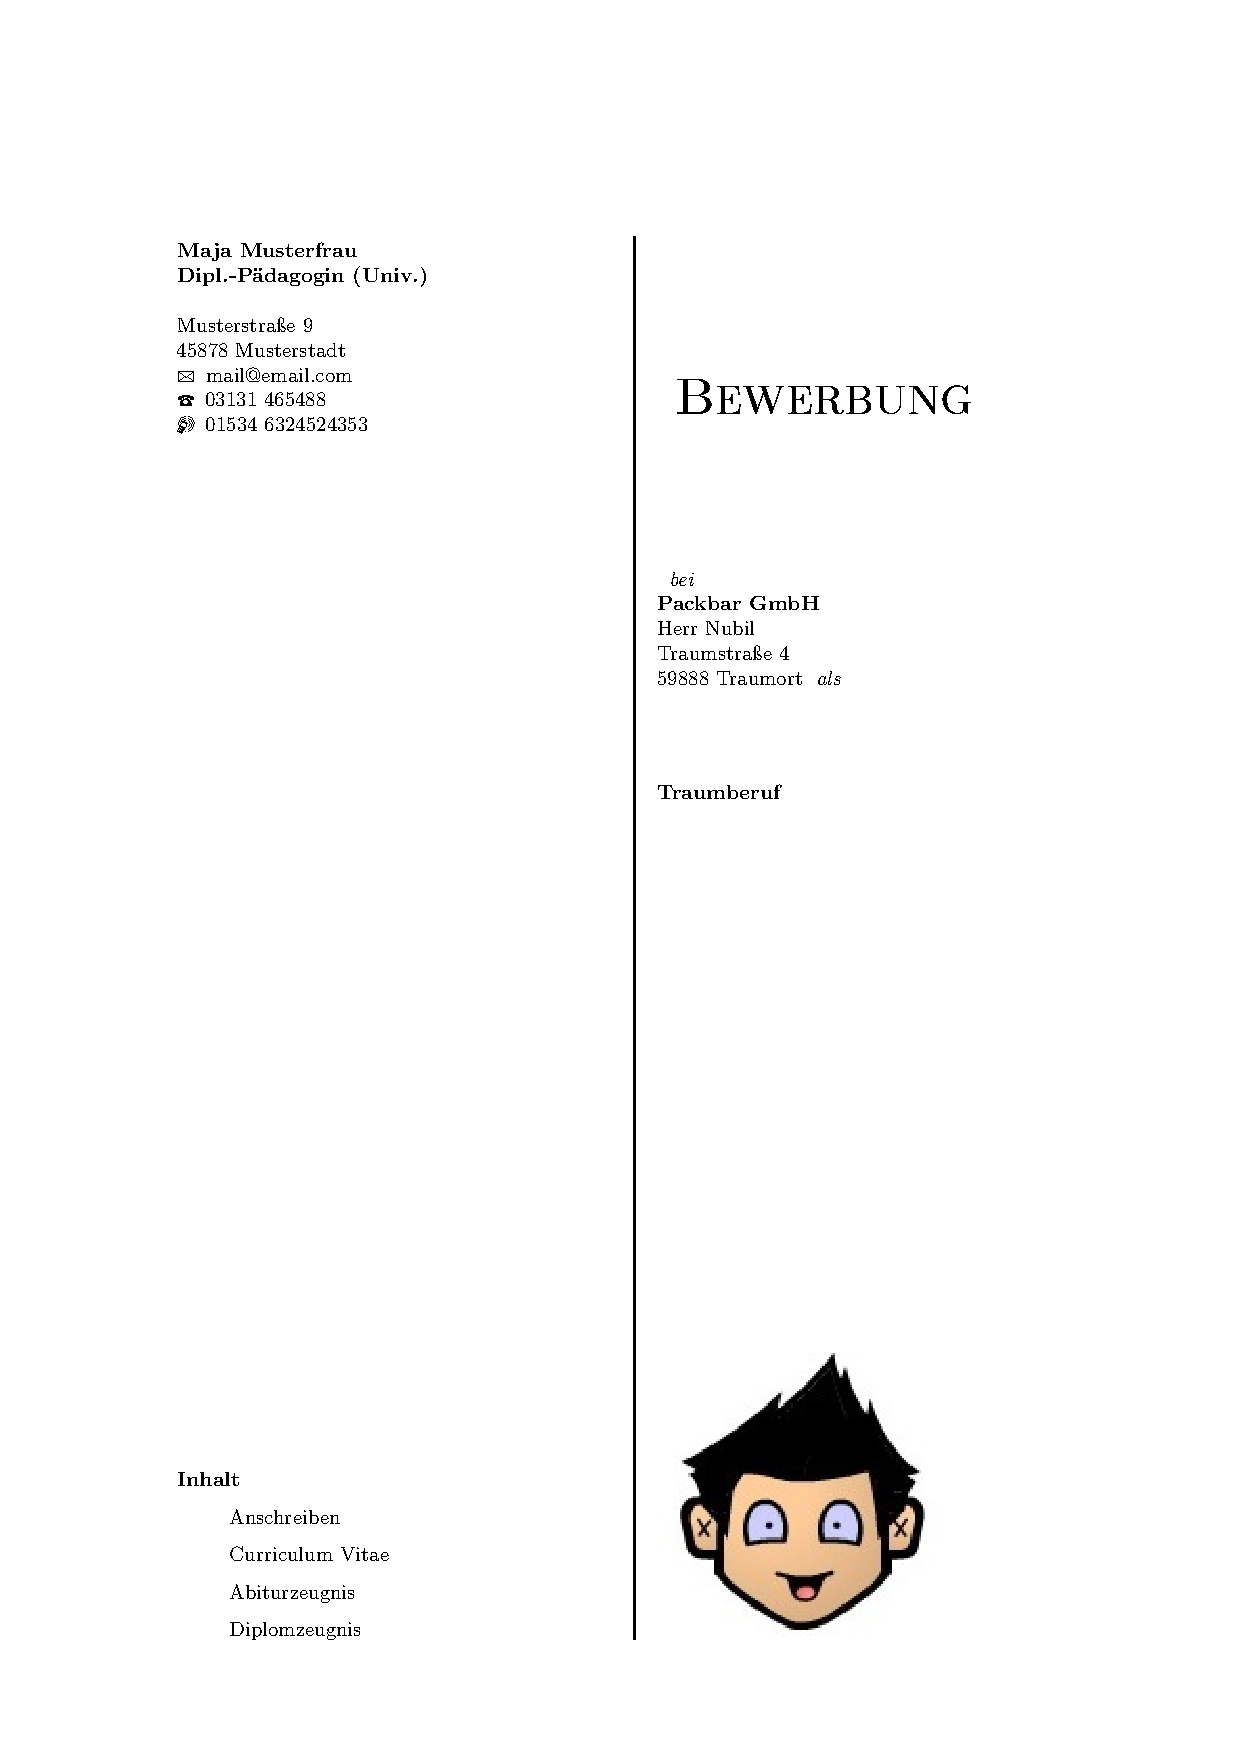
\includegraphics[page=1,scale=0.35]{bewerbung-example.pdf}}
%			\end{beispiel}
%
%			\subsubsection{Anschreiben}\label{sec:anschreiben}
%			Das Anschreiben einer Bewerbung stellt einen Brief an den potentiellen Arbeitgeber dar. Je
%			ordentlicher dieser Brief gesetzt ist, desto angenehmer fällt der Personalchefin das Lesen und
%			desto eher fallen wichtige Inhalte auf.
%
%			\DescribeEnv{anschreiben}
%			Innerhalb der Umgebung |{anschreiben}|\oarg{Anrede}\oarg{Enlarge} wird das Anschreiben
%			notiert.  Die gedruckte Anrede wird automatisch aus den Inhalten der Felder |firmaAnrede|
%			|firmaName| generiert.  Die Anpassung an den Genus der Anrede erfolgt über die Wahl von
%			\enquote{Frau} oder \enquote{Mann} in |firmaAnrede|. Alternativ kann das erste optionale
%			Argument mit dem richtigen Terminus von \enquote{geehrt} gesetzt werden. Dies kann hilfreich
%			sein, wenn die Anrede beispielsweise aus \enquote{Herr Dr.} besteht.
%
%			Als Faustregel für ein gutes Anschreiben wird häufig genannt, dass nicht mehr als eine DinA4
%			Seite verwendet werden sollte. Manchmal wird für einen einzelnen Satz eine neue Seite
%			angefangen, obwohl noch genügend leerer Platz zur Verfügung stünde. Hier versucht \LaTeX\
%			einen Fließtext zu optimieren. Um dem entgegenzuwirken kann als zweites optionales Argument
%			eine Größeneinheit, z.\,B. |2em|, angegeben werden. Dann wird \LaTeX\ versuchen das
%			Anschreiben um die angegebene Länge zu strecken.
%
%			Alle Optionen an |\documentclass{bewerbung}|, die nicht an diese Klasse gerichtet sind, werden
%			automatisch an |scrlttr2| \autocite[vgl.][]{scrlttr2} weitergereicht. Ansonsten werden
%			standardmäßig folgende Optionen geladen:
%			\begin{lstlisting}[gobble=9]
%				DIN, pagenumber=botright, backaddress=true, parskip=half,
%				fromalign=left, fromemail=true, fromfax=true,
%				fromphone=true, fromurl=false, fromalign=right,
%				fromlogo=false, fromrule=true, foldmarks=true,
%				paper=a4, fontsize=10pt,enlargefirstpage=true, firstfoot=false
%			\end{lstlisting}
%			Dadurch werden automatisch die deutschen DIN-Normen inklusive Schnittkanten gewählt. Als
%			Betreff wird »Bewerbung als |\meinBeruf|« gewählt. Über das Makro
%			|\setkomavar{subject}|\marg{Betreffstext} kann die Betreffszeile geändert	werden, sofern hier
%			ein anderer Betreff	gewünscht wird.
%
%			Sollten zusätzlich zum Lebenslauf weitere Anhänge angehangen werden, können diese mit dem
%			\refMacro{Anhang} in |config.inc| ausgewiesen werden.
%
%			\begin{beispiel}[bsp:anschreiben][Anschreiben]{Beispiel für ein Anschreiben}
%				\begin{lstlisting}[gobble=11]
%					\begin{anschreiben}
%						Hier kommt das Anschreiben hin
%					\end{anschreiben}	
%				\end{lstlisting}
%				\fbox{\includegraphics[page=2,scale=0.4]{bewerbung-example.pdf}}
%			\end{beispiel}
%			\FloatBarrier
%
%			\subsubsection{Lebenslauf}\label{sec:lebenslauf}
%			Jedem guten Bewerbungsschreiben sollte ein tabellarischer Lebenslauf angefügt werden.
%			Innerhalb dieses Dokuments wird nicht erläutert, welche Inhalte dort hinein gehören. Die
%			technische Realisierung basiert nahezu vollkommen auf der Arbeit von \citeauthorfull{komacv}
%			in \citetitle{komacv}. Einige Anpassungen und Ergänzungen wurden allerdings vor allem für das
%			Thema |classic| vorgenommen.  Die hier aufgeführten Erklärungen beziehen sich nur auf einen
%			kleinen Teil der Möglichkeiten von |komacv|. Alle Makros und Umgebungen wurden vollständig
%			portiert und sind verfügbar. Damit ist das Importieren eines Dokumentes mit der Klasse
%			|komacv| (evtl. unter Verwendung von |standalone|) möglich. In jedem Fall sollte bei
%			tiefergehenden Fragen die entsprechende Dokumentation konsultiert werden
%			\autocite[vgl.][]{komacv}.
%
%			\DescribeEnv{lebenslauf}
%			Die Umgebung |{lebenslauf}|\oarg{Listensymbol}\oarg{Addendum} erstellt einen Bereich in dem
%			sämtliche Befehle aus der Klasse |komacv| benutzt werden können. Über das erste optionale
%			Argument kann bei Bedarf das Listensymbol bei der Aufzählung von Einträgen durch Angabe von
%			|none| ausgeschaltet werden. Im zweiten optionalen Argument kann ein Addendum nach der
%			Unterschrift auf einer neuen Seite dem Lebenslauf angehangen werden. \textit{Achtung:} Um die
%			Register von \TeX\ nicht zu sprengen, dürfen hier zwar Sektionen und alle Befehle aus |komacv|
%			benutzt werden, jedoch dürfen keine Leerzeilen (im Zweifel auskommentieren) und erzwungene
%			Umbrüche mit |\\| (im Zweifel |\newline| verwenden) angegeben werden.
%
%			\DescribeMacro{\maktitle}
%			Das Makro |\maketitle| wurde angepasst und sollte zu Beginn des Lebenslaufs aufgerufen werden,
%			um den Titelkopf aus |komacv| aufzurufen.
%
%			\DescribeMacro{\makePerson}
%			Aus der Konfigurationsdatei werden die notwendigen Daten herausgelesen und ein passender
%			Eintrag für die eigene Person über |\makePerson| erzeugt. Dazu wird die Sektion
%			\enquote{Persönliche Angaben} mit |cvitem|s zu Name, Anschrift, Staatsangehörigkeit,
%			Geburtstdatum und eigenem Beruf angelegt.
%
%			Der Befehl führt zu keinem erzwungenen Umbruch. Somit kann die Sektion beliebig erweitert
%			werden.
%
%			\DescribeMacro{\cventry}
%			Mit |\cventry|\marg{Monat/Jahr}\marg{Bezeichnung}\marg{Ergänzung}\marg{Inhalt} kann
%			ein zeitlicher Eintrag nach |komacv| angelegt werden.
%
%			\DescribeMacro{\cvlistitem}
%			Um in einer Sektion eine Aufzählung zu führen, kann |\cvlistitem|\marg{Eintrag} verwendet
%			werden. Die letzten beiden Beschreibungen sollten ausführlicher den entsprechenden
%			Dokumentationen zu |komacv| entnommen werden.
%
%			\DescribeMacro{\cvlanguage}
%			\DescribeMacro{\cvitemwithcomment} 
%			Der normalen |komacv|-Klasse fehlt eine Möglichkeit Sprachkenntnisse anzugeben. Mit dem
%			Wrapper |\cvlanguage|\marg{Sprache}\marg{Kenntnisse}\marg{Kommentar} kann dies erledigt
%			werden. Letztlich wird dadurch ein |\cvitemwithcomment| nach selber Syntax erzeugt, der auch
%			für andere kommentierte Aufzählungen bzw. Einträge verwendet werden kann.
%
%			\begin{beispiel}[bsp:lebenslauf][Lebenslauf]{Beispiel für einen Lebenslauf}
%				\begin{lstlisting}[gobble=11]
%					\begin{lebenslauf}[none][]
%						\maketitle
%						\makePerson
%
%						\section{Studium}
%						\cventry{03/13}{Abschluss: Dipl.-Pädagogin (Univ.)}{}{}{}{}
%
%						\section{Führerschein}
%						\cvlistitem{Klasse B (eigener PKW)}
%
%						\section{Sprachen}
%						\cvlanguage{Deutsch}{Muttersprache}{}
%						\cvlanguage{Englisch}{gut}{}
%					\end{lebenslauf}
%				\end{lstlisting}
%				\fbox{\includegraphics[page=3,scale=0.4]{bewerbung-example.pdf}}
%			\end{beispiel}
%			\FloatBarrier
%
%			\subsubsection{Anhang}\label{sec:anhang}
%			Gerade bei Bewerbungen per E"~Mail ist es häufig notwendig digitale Kopien von Zeugnissen,
%			Zertifikaten usw. mitzuschicken. In jedem Fall sollten entsprechende Anhänge bei einer
%			schriftlichen Einreichung als Anhang auf dem Deckblatt und dem Anschreiben ausgewiesen werden.
%			\DescribeMacro{\Anhang}
%			Dazu sollte das Makro |\Anhang| verwendet werden (vgl. \refMacro{Anhang}).
%		 
%			Um Anhänge nicht händisch an das PDF anzufügen, kann dies mit dem Paket \citetitle{pdfpages}
%			von \citeauthorfull{pdfpages} sehr elegant innerhalb des \TeX-Dokuments geschehen. Hier werden
%			dazu nur kleine Ausschnitte dieses mächtigen Werkzeugs dargestellt. Prinzipiell ist damit jede
%			nur erdenkliche Einbindung von Dateien im PDF"~Format möglich	\autocite[vgl.][]{pdfpages}.
%
%			\DescribeMacro{\includepdf}
%			Mit dem Befehl |\includepdf|\oarg{Optionen}\marg{Dateien} können PDF-Dateien beliebigen
%			Formats und Länge eingebunden werden. Bei Angabe ohne Optionen wird automatisch die erste
%			Seite im \textit{Vollbildmodus} über eine gesamte Seite in die Bewerbungsmappe integriert.
%
%			Um etwa ein mehrseitiges Diplomzeugnis einzubinden, ist der Aufruf
%			\begin{lstlisting}[gobble=9,numbers=none]
%				\includepdf[pages=-]{diplomzeugnis.pdf}
%			\end{lstlisting} 
%			sinnvoll. Die Option |pages=-|
%			weist |includepdf| dabei an, alle Seiten der Datei |diplomzeugnis.pdf| zu verwenden. Hier wäre
%			auch eine beliebige alphanumerische Angabe, etwa |2-9|, möglich. Das Format aller Seiten wird
%			automatisch auf das gewählte Format (DinA4) der Mappe skaliert. Über die Option |scale=0.5|
%			kann dies bei Bedarf angepasst werden.
%
%			\DescribeMacro{\includepdfmerge}
%			Sofern die anzuhängenden Seiten in einem Querformat vorliegen, kann über die Option
%			|landscape| automatisch gedreht werden. Zusätzlich kann über die Option |angle=270| auch die
%			Datei selbst vor dem Einbinden um einen beliebigen Winkel gedreht werden. Mehrere Dateien
%			können mit den selben Optionen in einem Aufruf über |\includepdfmerge| eingefügt werden:
%
%			\begin{lstlisting}[gobble=9,numbers=none]
%				\includepdfmerge[pages=-,landscape,angle=270]%
%												{Abiturzeugnis1.pdf,Abiturzeugnis2.pdf}
%			\end{lstlisting}
%
%			Eventuell kann auch die Option |nup=XxY| hilfreich sein. Dadurch werden jeweils mehrere
%			Seiten eines mehrseitigen Dokumentes zusammen auf einer Seite mit |X|"~Seiten pro Länge und
%			|Y|"~Seiten pro Höhe dargestellt.  Für weitere Informationen sei auf die Paketdokumentation
%			verwiesen \autocite[vgl.][]{pdfpages}.
%
%			\begin{beispiel}[bsp:bewerbungsmappe][Vollständige Bewerbungsmappe]{%
%					Beispiel für den Quellcode einer vollständigen Bewerbungsmappe}
%				\begin{lstlisting}[gobble=11,multicols=2,title={Datei: \texttt{bewerbung.tex}},%
%					xleftmargin=5pt,linewidth=0.95\columnwidth]
%					\documentclass[%
%					 lebenslaufColor=light-gray,%
%					 %lebenslaufStyle=classic,
%					 idPlain%
%					]{bewerbung}
%					\usepackage[utf8]{inputenc}
%					\usepackage[T1]{fontenc}
%					\usepackage[ngerman]{babel}
%					% zusätzliche 
%					% Farbdefinitionen:
%					\definecolor{light-gray}%
%						{gray}{0.6}
%					\definecolor{titlecolor}%
%						{gray}{0.62}
%					\definecolor{addresscolor}%
%						{gray}{0.45}
%
%					\begin{document}
%						\begin{anschreiben}
%							Hier kommt das 
%							Anschreiben hin
%						\end{anschreiben}	
%
%						\begin{lebenslauf}[none][]
%							\maketitle
%							\makePerson
%
%							\section{Studium}
%							\cventry{03/13}{%
%								Abschluss: %
%								Dipl.-Pädagogin %
%								(Univ.)%
%							}{}{}{}{}
%
%							\section{Führerschein}
%							\cvlistitem{%
%								Klasse B %
%								(eigener PKW)}
%
%							\section{Sprachen}
%							\cvlanguage{Deutsch}{%
%								Muttersprache}{}
%							\cvlanguage{Englisch}{%
%								gut}{}
%						\end{lebenslauf}
%					\ end{document}
%				\end{lstlisting}
%				
%				\begin{lstlisting}[gobble=11,multicols=2,title={Datei: \texttt{config.inc}},%
%					xleftmargin=5pt,linewidth=0.95\columnwidth]
%					\Name{Musterfrau}
%					\Vorname{Maja}
%					\Street{Musterstraße 9}
%					\Plz{45878}
%					\Stadt{Musterstadt}
%					\MeinBeruf{Dipl.-Pädagogin%
%					 	(Univ.)}
%					\EMail{mail@email.com}
%					\Tel{03131~465488}
%					\Mobile{01534~6324524353}
%					\Sta{deutsch}
%					\GebDatum{31.02.1990}
%					\ID{47}
%					\Anhang{%
%						Abiturzeugnis.\newline 
%						Diplomzeugnis.
%					}{%
%						\item Abiturzeugnis
%						\item Diplomzeugnis
%					}
%				\end{lstlisting}
%				
%				\begin{lstlisting}[gobble=11,language=bash,title={Datei: \texttt{anschrift.csv}}]
%					ID,KW,Datum,Firma,FirmaAnrede,FirmaName,Str,PLZ,Ort,Stelle, Rueckmeldung,Sonstiges
%					2,13,26.09.15,Packisbar GmbH,Frau,Nauti,Traumstraße 19,59888,Traumort,Traumberuf,n,n
%					1,12,14.09.15,Packbar GmbH,Herr,Nubil,Traumstraße 4,59888,Traumort,Traumberuf,n,n
%				\end{lstlisting}
%			\end{beispiel}
%
%			\begin{landscape}
%				\begin{beispiel}[bsp:bewerbungsmappepdf][Ergebnis einer vollständigen Mappe]{%
%						Ergebnis des Quellcodes aus	\prettyref{bsp:bewerbungsmappe}}
%					\begin{minipage}{0.5\textwidth}
%						\fbox{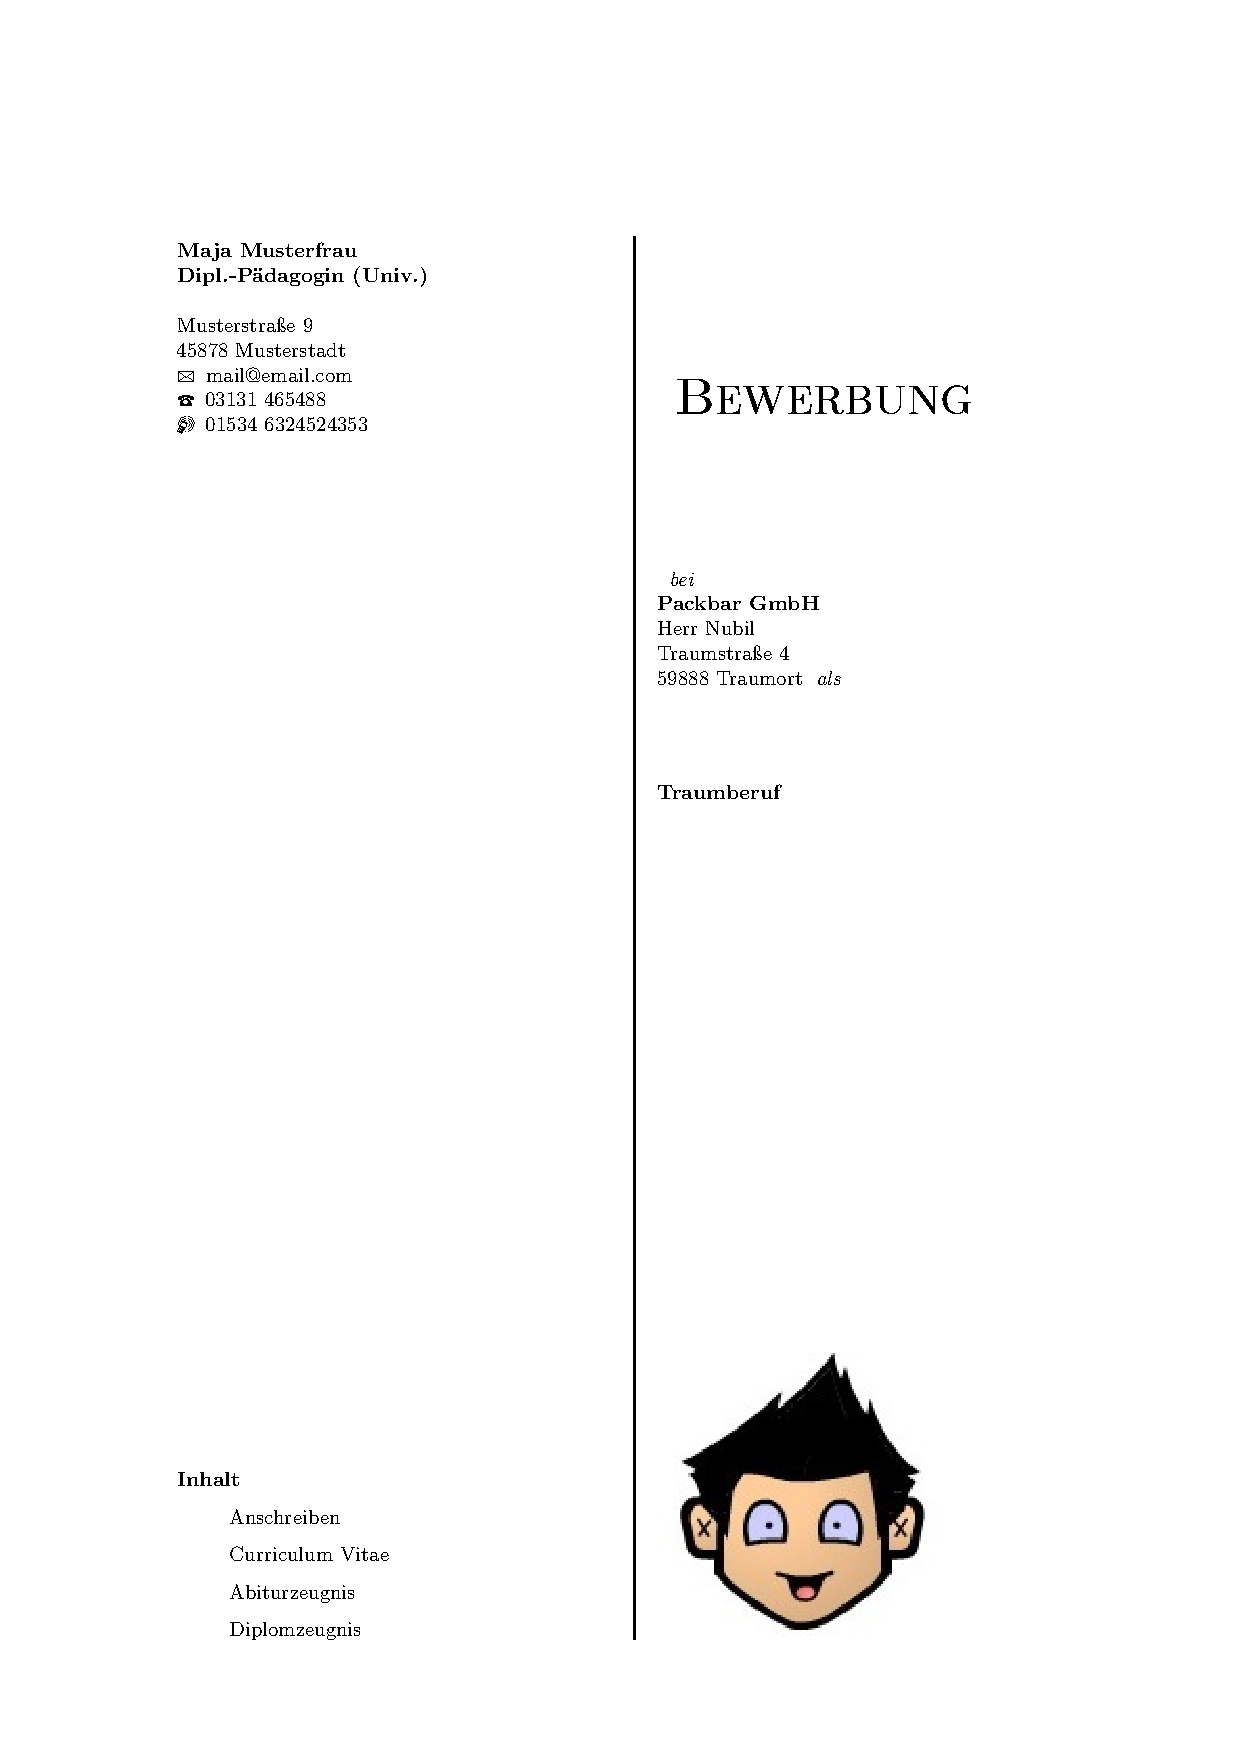
\includegraphics[page=1,width=\textwidth]{bewerbung-example.pdf}}
%					\end{minipage}\quad\ 
%					\begin{minipage}{0.5\textwidth}
%						\fbox{\includegraphics[page=2,width=\textwidth]{bewerbung-example.pdf}}
%					\end{minipage}\quad\ 
%					\begin{minipage}{0.5\textwidth}
%						\fbox{\includegraphics[page=3,width=\textwidth]{bewerbung-example.pdf}}
%					\end{minipage}
%				\end{beispiel}
%			\end{landscape}
%			\FloatBarrier
%		\subsection[Dokumentationstabelle]{Erstellung einer	Dokumentationstabelle}
%		\label{sec:dokutabelle}
%		Die Agentur für Arbeit verlangt von ihren \textit{Kunden} typischerweise den Nachweis über die
%		Vertragstreue.  Im Klartext heißt dies, dass Menschen eine Vorgabe an Bewerbungen pro Woche oder
%		Monat und die Bindung an das Bewerben auf jede von der Agentur für Arbeit vorgeschlagene Stelle
%		unterschreiben müssen, um den Almosen Grundsicherung, auch HartzIV genannt, zu erhalten. Wird
%		gegen diese Auflagen verstoßen ist mit Abzügen der Grundsicherung zu rechnen. Da Kunden
%		typischerweise nicht zu trauen ist, müssen diese über ihre Bewerbungsversuche detailliert
%		Aufschluss geben.
%
%		Um sich bei dieser oftmals lästigen Dokumentationsarbeit Zeit zu sparen, entstand die Grundidee
%		zu dieser Zusammenstellung. Dafür wird eine Tabelle automatisiert erstellt, indem eine csv-Datei
%		(vgl. \prettyref{sec:bewerbung}) ausgewertet wird. Die Klasse |argetabelle| ermöglicht das Setzen
%		solch einer Tabelle auch über mehrere Seiten hinweg.
%
%		Der Klasse können dabei Optionen an |scrartcl| weiter gereicht werden. Allerdings ist es nicht
%		ratsam die Dimensionen inkl. Ausrichtung der Seite zu ändern, da die Skalierung der Tabelle
%		\DescribeMacro{\argetballe}
%		(noch) absolut ist. Die Tabelle wird über den Aufruf des Makros |\argetabelle|\oarg{Datei}
%		gesetzt. Sofern die Datei mit den Anschriften zu den Bewerbungen nicht als |anschrift.csv|
%		benannt wurde, kann diese im optionalen Argument angegeben werden.
%
%		\textit{Hinweis:} Die Tabelle wird immer in der Reihenfolge der Zeilen in der angegebenen
%		csv"~Datei gesetzt. Das Feld ID ist hierbei irrelevant.
%
%		\begin{beispiel}[bsp:dokutabelle]{Beispiel für das Setzen der Dokumentationstabelle}
%			\begin{lstlisting}[gobble=9,title={Datei: \texttt{argetabelle.tex}}]
%				\documentclass[11pt,a4paper]{argetabelle}
%				\usepackage[utf8]{inputenc}
%				\usepackage[T1]{fontenc}
%				\usepackage[ngerman]{babel}
%				\begin{document}
%					\argetabelle
%				\ end{document}
%			\end{lstlisting}
%				
%			\begin{lstlisting}[gobble=9,language=bash,title={Datei: \texttt{anschrift.csv}}]
%				ID,KW,Datum,Firma,FirmaAnrede,FirmaName,Str,PLZ,Ort,Stelle, Rueckmeldung,Sonstiges
%				2,13,26.09.15,Packisbar GmbH,Frau,Nauti,Traumstraße 19,59888,Traumort,Traumberuf,n,n
%				1,12,14.09.15,Packbar GmbH,Herr,Nubil,Traumstraße 4,59888,Traumort,Traumberuf,n,n
%			\end{lstlisting}
%
%			\fbox{
\includegraphics[width=0.95\textwidth,page=1,viewport=52.815022 610 542.460991
%				771.024000]{argetabelle-example.pdf}}
%			\vspace{1.4em}
%		\end{beispiel}
%
%	\clearpage
%	\addcontentsline{toc}{section}{Literatur}
%	\printbibliography
%
%
%\StopEventually{}
%\section{Implementation}
%\iffalse
%    \begin{macrocode}
%<*bewerbung-cv-casual.sty>
%    \end{macrocode}
%\fi
%    \begin{macrocode}
\NeedsTeXFormat{LaTeX2e}[1999/12/01]
\ProvidesPackage{bewerbung-cv-casual} %
    [2015/07/14 v1.1 theme für bewerbungen basiert auf komacv-casual]
	 %% this file is based on komacv-casual.sty from Salome Södergran
	 %% every change is marked by
	 %%  %% ahilbig begin
	 %%     CHANGE
	 %%  %% ahilbig end
\addtokomafont{firstnamefont}{\sffamily\fontsize{38}{40}}
\addtokomafont{acadtitlefont}{\sffamily}
\addtokomafont{addressfont}{\sffamily\small}
\addtokomafont{hintfont}{\sffamily}
\newsavebox\@fboxa
\newsavebox\@fboxb
%    \end{macrocode}
%
% \begin{macro}{\@sboxa}
%    \begin{macrocode}
\newcommand*\@sboxa[1]{\sbox\@fboxa{#1}}
%    \end{macrocode}
% \end{macro}
%
%
% \begin{macro}{\@sboxb}
%    \begin{macrocode}
\newcommand*\@sboxb[1]{\sbox\@fboxb{#1}}
%    \end{macrocode}
% \end{macro}
%
%
% \begin{macro}{\@uboxa}
%    \begin{macrocode}
\newcommand*\@uboxa{\usebox\@fboxa}
%    \end{macrocode}
% \end{macro}
%
%
% \begin{macro}{\@uboxb}
%    \begin{macrocode}
\newcommand*\@uboxb{\usebox\@fboxb}
%    \end{macrocode}
% \end{macro}
%
%
% \begin{macro}{\@flushf}
%    \begin{macrocode}
\newcommand*\@flushf{\strut\@uboxa\@sboxa{}\@sboxb{}}
%    \end{macrocode}
% \end{macro}
%
%
% \begin{macro}{\addtofooter}
%    \begin{macrocode}
\newcommand*\addtofooter[2][\@fsymbol]{%
  \@sboxb{\@uboxa{}#1#2}%
  \settowidth\@fboxwidth{\@uboxb}%
  \ifdimgreater{\@footerwidth}{\@fboxwidth}{%
    \@sboxa{\@uboxb}
  }{%
    \@flushf\\
    \@sboxa{#2}
    \@sboxb{#2}
  }
}
%    \end{macrocode}
% \end{macro}
%
%    \begin{macrocode}
	\ifdimequal{\footerwidth}{0pt}{}{%
		\setlength\@footerwidth{\footerwidth}%
	}
  \defpagestyle{footer}
  {{}{}{}}% head definition (empty)
  {% foot definition
    {}{}% definition for twoside layout
    {% definition for oneside layout
      \hspace*{\fill}%
      \parbox{\@footerwidth}{%
        \centering%
        \color{@addresscolor}\usekomafont{addressfont}%
        \ifdefempty{\addressstreet}{}{%
          \addtofooter[]{\@addresssymbol\addressstreet}%
          \ifdefempty{\addresscity}{}{%
            \addtofooter[~--~]{\addresscity}}}%
        \ifdefempty{\mobile}{}{%
          \addtofooter{\@mobilesymbol\mobile}}%
        \ifdefempty{\phonenr}{}{%
          \addtofooter{\@phonesymbol\phonenr}}
        \ifdefempty{\faxnr}{}{%
          \addtofooter{\@faxsymbol\faxnr}}%
        \ifdefempty{\email}{}{%
          \addtofooter{\@emailsymbol\emaillink{\email}}}
        \ifdefempty{\homepage}{}{%
          \addtofooter{\@homepagesymbol\httplink{\homepage}}}%
        \ifdefempty{\extrainfo}{}{%
          \addtofooter{\extrainfo}}\@flushf%
      }% Ende parbox
      \hspace*{\fill}%
      \makebox[0pt][r]{\pagemark/\totalpagemark}
    }% end definition onesided layout
  }% end footer definition
%    \end{macrocode}
%
% \begin{macro}{\@cvtitlecasual}
%    \begin{macrocode}
\providecommand\@cvtitlecasual{%
\newbox{\@picbox}
\savebox{\@picbox}{%
  \ifundef{\@photoname}{}{% with picture:
    \ifthenelse{%
      \equal{\@photoframe}{frame} \OR
      \equal{\@photoframe}{mframe}
    }{% with frame:
      \fcolorbox{@framecolor}{@framebackcolor}{%
        \includegraphics[width=\@photowidth]{\@photoname}%
      }% end fcolorbox
    }{% without frame:
      \includegraphics[width=\@photowidth]{\@photoname}%
    }% end ifdefstring frame
  }% end ifundef photoname
}% end savebox picbox
\settowidth\@titlepicwidth{\usebox{\@picbox}}
\setlength\@titlenamewidth{\textwidth-\@titlesepwidth-\@titlepicwidth}
  \usebox{\@picbox}%
  \hspace*{\@titlesepwidth}%
  \parbox[b]{\@titlenamewidth}{%
		\raggedleft{\firstnamestyle\firstname}%
    ~{\familynamestyle\familyname}\\
    \raggedleft\color{@firstnamecolor}\rule{%
			\@titlenamewidth}{.25ex}\par
  }% end parbox
  \vspace{\@aftertitlevspace}
  %% optional acadtitle
  \ifdefempty{\acadtitle}{}{%
    \raggedleft\acadtitlestyle{\acadtitle}}\\[2.5em]%
  %% optional quote
  \ifdefempty{\cvquote}{}{%
    {\centering
      \begin{minipage}{\@quotewidth}%
        \centering\quotestyle{\cvquote}
      \end{minipage}\\[\@afterquotevspace]%
    }
  }%
}% end @cvtitle-casual
\AtBeginDocument{%
  \thispagestyle{footer}
} % end AtBeginDocument
%    \end{macrocode}
% \end{macro}
%
%
% \begin{macro}{\section}
%    \begin{macrocode}
\renewcommand{\section}[1]{\@cvbarsection{#1}}
%    \end{macrocode}
% \end{macro}
%
%
% \begin{macro}{\subsection}
%    \begin{macrocode}
\renewcommand{\subsection}[1]{\@cvbarsubsection{#1}}
%    \end{macrocode}
% \end{macro}
%
%\iffalse
%    \begin{macrocode}
%</bewerbung-cv-casual.sty>
%    \end{macrocode}
%\fi
%\iffalse
%    \begin{macrocode}
%<*bewerbung-cv-classic.sty>
%    \end{macrocode}
%\fi
%    \begin{macrocode}
\NeedsTeXFormat{LaTeX2e}[1999/12/01]
\ProvidesPackage{bewerbung-cv-classic} %
    [2015/07/14 v1.1 theme für bewerbungen basiert auf komacv-classic]
	%% this file is based on komacv-classic.sty from Salome Södergran
	%% every change is marked by
	%%  %% ahilbig begin
	%%     CHANGE
	%%  %% ahilbig end
\addtokomafont{firstnamefont}{\sffamily}
\addtokomafont{acadtitlefont}{\sffamily}
\addtokomafont{addressfont}{\sffamily}
\addtokomafont{hintfont}{\sffamily}
\AtEndPreamble{%
 %AtBeginDocument{
%    \end{macrocode}
% mframepicshift
%    \begin{macrocode}
  \ifdimequal{\mframepicshift}{0pt}{%
    \setlength\@mframepicshift{.5\@photowidth+\@fboxextra}
  }{%
    \setlength\@mframepicshift{\mframepicshift}
  }
} % end AtBeginDocument
%    \end{macrocode}
%
% \begin{macro}{\@cvtitleclassic}
%    \begin{macrocode}
\providecommand\@cvtitleclassic{%
 %% set cs{@titlenamemaxwidth| to the full name length
 %% , capped by cs{@titlenamemaxwidth|
\setlength{\@titlenamemaxwidth}{.525\textwidth}
\settowidth{\@titlenamefullwidth}{%
	\firstnamestyle{\firstname~}\familynamestyle{\familyname}}
 \ifdimless{\@titlenamemaxwidth}{\@titlenamefullwidth}{%
   \setlength{\@titlenamewidth}{\@titlenamemaxwidth}
 }{%
   \setlength{\@titlenamewidth}{\@titlenamefullwidth}
 }
%    \end{macrocode}
% set titlenamedetailswidth
%    \begin{macrocode}
\setlength{\@titledetailswidth}{%
	\textwidth-\@titlenamewidth-\@titlesepwidth}%
\ifundef{\@photoname}{}{% else
  \ifdefstring{\@photoframe}{frame}{%
    \setlength{\@titledetailswidth}{%
			\@titledetailswidth-\@photowidth-2\@fboxextra}
  }{% else
  \ifdefstring{\@photoframe}{mframe}{%
    \setlength{\@titledetailswidth}{%
			\@titledetailswidth-\@mframepicshift}%
  }{}%
}%
}%
%    \end{macrocode}
% name and title
%    \begin{macrocode}
  \begin{minipage}[b]{\@titlenamewidth}%
%    \end{macrocode}
%% ahilbig begin
%    \begin{macrocode}
    \firstnamestyle{\firstname}\\ %
    \familynamestyle{\familyname}%
    \ifdefempty{\acadtitle}{}{%
      \\[1.25em]\acadtitlestyle{\acadtitle}}%
     \\[1.25em]\titlestyle{\lebenslaufTitel}%
  \end{minipage}%
%    \end{macrocode}
% optional data
%    \begin{macrocode}
  \begin{minipage}[b]{\@titledetailswidth}%
    \raggedleft\addressstyle{%
    \ifdefempty{\addressstreet}{}{%
      \@titledetailsnewline%
      \@addresssymbol\addressstreet%
      \ifdefempty{\addresscity}{}{%
        \@titledetailsnewline\addresscity}}%
    \ifdefempty{\mobile}{}{%
      \@titledetailsnewline\@mobilesymbol~\mobile}%
    \ifdefempty{\phonenr}{}{%
      \@titledetailsnewline\@phonesymbol~\phonenr}%
    \ifdefempty{\faxnr}{}{%
      \@titledetailsnewline\@faxsymbol~\faxnr}%
    \ifdefempty{\email}{}{%
      \@titledetailsnewline\@emailsymbol\emaillink{\email}}%
    \ifdefempty{\homepage}{}{%
      \@titledetailsnewline\@homepagesymbol\httplink{\homepage}}%
    \ifdefempty{\extrainfo}{}{%
      \@titledetailsnewline\extrainfo}%
  }%
%    \end{macrocode}
%% ahilbig end
%    \begin{macrocode}
  \end{minipage}%
%    \end{macrocode}
% optional photo
%    \begin{macrocode}
  \ifundef{\@photoname}{}{% with picture:
    \hspace*{\@titlesepwidth}%
    \ifthenelse{%
      \equal{\@photoframe}{frame} \OR
      \equal{\@photoframe}{mframe}
    }{% with frame:
      \begin{minipage}[b]{\@photowidth}%
        \fcolorbox{@framecolor}{@framebackcolor}{%
          \includegraphics[width=\@photowidth]{\@photoname}}%
      \end{minipage}}{% without frame:
      \begin{minipage}[b]{\@photowidth}
        \includegraphics[width=\@photowidth]{\@photoname}
      \end{minipage}}}
\\[\@aftertitlevspace]
%    \end{macrocode}
% optional quote
%    \begin{macrocode}
  \ifundef{\cvquote}{}{%
    \centering
      \begin{minipage}{\@quotewidth}%
        \centering\quotestyle{\cvquote}%
      \end{minipage}\\[\@afterquotevspace]%
  }%
}
%    \end{macrocode}
% \end{macro}
%
%
% \begin{macro}{\section}
%    \begin{macrocode}
\renewcommand*{\section}[1]{\@cvbarsection{#1}}
%    \end{macrocode}
% \end{macro}
%
%
% \begin{macro}{\subsection}
%    \begin{macrocode}
\renewcommand{\subsection}[1]{\@cvbarsubsection{#1}}
%    \end{macrocode}
% \end{macro}
%
%\iffalse
%    \begin{macrocode}
%</bewerbung-cv-classic.sty>
%    \end{macrocode}
%\fi
%\iffalse
%    \begin{macrocode}
%<*bewerbung-cv-oldstyle.sty>
%    \end{macrocode}
%\fi
%    \begin{macrocode}
\NeedsTeXFormat{LaTeX2e}[1999/12/01]
\ProvidesPackage{bewerbung-cv-oldstyle} %
    [2015/07/14 v1.1 theme für bewerbungen basiert auf komacv-oldstyle]
	%% this file is based on komacv-oldstyle.sty from Salome Södergran
	%% every change is marked by
	%%  %% ahilbig begin
	%%     CHANGE
	%%  %% ahilbig end
\KOMAoptions{DIV=15}
\setlength{\hintscolwidth}{3cm}
\addtokomafont{addressfont}{\small}
\addtokomafont{hintfont}{\bfseries}
\setkomafont{section}{\Large\bfseries\upshape}
\setkomafont{subsection}{\large\bfseries\itshape}
\colorlet{addresscolor}{gray}
%    \end{macrocode}
%
% \begin{macro}{\listitemsymbol}
%    \begin{macrocode}
\renewcommand*{\listitemsymbol}{\labelitemi~}
%    \end{macrocode}
% \end{macro}
%
%
% \begin{macro}{\addresssymbol}
%    \begin{macrocode}
\renewcommand*{\addresssymbol}{}
%    \end{macrocode}
% \end{macro}
%
%
% \begin{macro}{\mobilesymbol}
%    \begin{macrocode}
\renewcommand*{\mobilesymbol}{\textbf{M}~}
%    \end{macrocode}
% \end{macro}
%
%
% \begin{macro}{\phonesymbol}
%    \begin{macrocode}
\renewcommand*{\phonesymbol}{\textbf{T}~}
%    \end{macrocode}
% \end{macro}
%
%
% \begin{macro}{\faxsymbol}
%    \begin{macrocode}
\renewcommand*{\faxsymbol}{\textbf{F}~}
%    \end{macrocode}
% \end{macro}
%
%
% \begin{macro}{\emailsymbol}
%    \begin{macrocode}
\renewcommand*{\emailsymbol}{\textbf{E}~}
%    \end{macrocode}
% \end{macro}
%
%
% \begin{macro}{\homepagesymbol}
%    \begin{macrocode}
\renewcommand*{\homepagesymbol}{}
%    \end{macrocode}
% \end{macro}
%
%    \begin{macrocode}
\setlength{\infocolwidth}{3.5cm}
\setlength{\sepinfocolwidth}{2em}
%    \end{macrocode}
%
% \begin{macro}{\@infocontent}
%    \begin{macrocode}
\providecommand\@infocontent{%
    \ifdefempty{\addressstreet}{}{%
      \@titledetailsnewline%
      \@addresssymbol\addressstreet%
      \ifdefempty{\addresscity}{}{%
        \@titledetailsnewline\addresscity}}%
    \ifdefempty{\mobile}{}{%
      \@titledetailsnewline\@mobilesymbol~\mobile}%
    \ifdefempty{\phonenr}{}{%
      \@titledetailsnewline \@phonesymbol\phonenr}%
    \ifdefempty{\faxnr}{}{%
      \@titledetailsnewline\@faxsymbol\faxnr}%
    \ifdefempty{\email}{}{%
      \@titledetailsnewline\@emailsymbol\emaillink{\email}}%
    \ifdefempty{\homepage}{}{%
      \@titledetailsnewline\@homepagesymbol\httplink{\homepage}}%
    \ifdefempty{\extrainfo}{}{%
      \@titledetailsnewline\extrainfo}%
} % end @infocontent
 \providecommand{\@makeinfo}{%
   \newbox{\@infobox}%
   \savebox{\@infobox}{%
     \parbox[b]{\@infocolwidth}{%
%    \end{macrocode}
% put the first line on the same 
% baseline as the first sectiontitle:
%    \begin{macrocode}
       {\usekomafont{section}
         \vspace*{1.6ex}
       }
       \raggedleft\addressstyle{%
         \@infocontent%
       }
     }% end parbox
   } % end savebox @infobox%
   \newlength{\@infoheight}%
   \setlength{\@infoheight}{%
     \totalheightof{\usebox{\@infobox}}%
   }%
   \usebox{\@infobox}\vspace*{-\@infoheight}%
   \par\nointerlineskip%
   \vspace*{-\parskip}%
   \vspace*{-\@aftersecvspace}
 }% end \providecommand @makeinfo
  \providecommand{\@cvtitleoldstyle}{%
%    \end{macrocode}
% optional picture box
%    \begin{macrocode}
    \newbox{\@picbox}
    \savebox{\@picbox}{%
      \ifundef{\@photoname}{}{% with picture:
        \ifthenelse{%
          \equal{\@photoframe}{frame} \OR
          \equal{\@photoframe}{mframe}
        }{% with frame:
          \fcolorbox{@framecolor}{@framebackcolor}{%
            \includegraphics[width=\@photowidth]{\@photoname}%
          }% end fcolorbox
        }{% without frame:
          \includegraphics[width=\@photowidth]{\@photoname}%
        }% end ifdefstring frame
      }% end ifundef photoname
    }% end savebox picbox
    \settowidth\@titlepicwidth{\usebox{\@picbox}}
    \setlength\@titlenamewidth{%
			\textwidth-\@titlesepwidth-\@titlepicwidth}
    \begin{minipage}[b]{\@titlenamewidth}%
      \firstnamestyle{\firstname}\ %
      \familynamestyle{\familyname}%
      \ifdefempty{\acadtitle}{}{%
        \\[1.25em]\acadtitlestyle{\acadtitle}}%
    \end{minipage}%
%    \end{macrocode}
% optional photo
%    \begin{macrocode}
      \usebox{\@picbox}%
      \\[\@aftertitlevspace]%
%    \end{macrocode}
% optional quote
%    \begin{macrocode}
    \ifdefempty{\cvquote}{}{%
      {\centering%
        \begin{minipage}{\@quotewidth}%
          \centering\quotestyle{\cvquote}%
        \end{minipage}\\[\@afterquotevspace]%
      }%
    }%
%    \end{macrocode}
% address info box
%    \begin{macrocode}
     \@makeinfo
\par
\begin{addmargin}[\komacvinfocolextrawidth]{0pt}
  } % end @cvtitleoldstyle
\AtEndDocument{%
\end{addmargin}
}
%    \end{macrocode}
% \end{macro}
%
%
% \begin{macro}{\section}
%    \begin{macrocode}
\renewcommand{\section}[1]{\@cvsimplesection{#1}}
%    \end{macrocode}
% \end{macro}
%
%
% \begin{macro}{\subsection}
%    \begin{macrocode}
\renewcommand{\subsection}[1]{\@cvsimplesubsection{#1}}
%    \end{macrocode}
% \end{macro}
%
%
% \begin{macro}{\cvitem}
%    \begin{macrocode}
\renewcommand*{\cvitem}[3][\@afterelementsvspace]{%
  \begin{tabular}{%
      @{}p{\@maincolwidth}%
      @{\hspace{\@sepcolwidth}}p{\@hintscolwidth}@{}%
    }%
    {#3} & \raggedright\hintstyle{#2}%
  \end{tabular}\\[#1]%
}
%    \end{macrocode}
% \end{macro}
%
%
% \begin{macro}{\cvdoubleitem}
%    \begin{macrocode}
\renewcommand*{\cvdoubleitem}[5][\@afterelementsvspace]{%
 \cvitem[#1]{#4}{%
   \begin{minipage}[t]{\@dbitemmaincolwidth}#3\end{minipage}%
   \hspace*{\@sepcolwidth}%
   \begin{minipage}[t]{\@hintscolwidth}%
     \noindent\raggedleft\hintstyle{#2}
   \end{minipage}%
   \hspace*{\@sepcolwidth}%
   \begin{minipage}[t]{\@dbitemmaincolwidth}%
     \noindent #5
   \end{minipage}%
 }%
}
%    \end{macrocode}
% \end{macro}
%
%\iffalse
%    \begin{macrocode}
%</bewerbung-cv-oldstyle.sty>
%    \end{macrocode}
%\fi
%\iffalse
%    \begin{macrocode}
%<*bewerbung-cv.sty>
%    \end{macrocode}
%\fi
%    \begin{macrocode}
\NeedsTeXFormat{LaTeX2e}[1999/12/01]
\ProvidesPackage{bewerbung-cv} %
    [2015/07/14 v1.1 Importierung der Klasse koma-cv %
		 für bewerbungen]
	%% this file is based on komacv.cls from Salome Södergran
	%% every change is marked by
	%%  %% ahilbig begin
	%%     CHANGE
	%%  %% ahilbig end
%    \end{macrocode}
%
% \begin{macro}{\mycolor}
%    \begin{macrocode}
\providecommand*\mycolor{blue}
%    \end{macrocode}
% \end{macro}
%
%% ahilbig begin
%\iffalse
%%\RequirePackage{ifthen,kvoptions,calc}
%%\SetupKeyvalOptions{%
%%family=komacv,%
%%prefix=komacv@,%
%%setkeys=\kvsetkeys%
%%}
%%\DeclareStringOption[mycolor]{color}[mycolor]
%%\DeclareStringOption[x11names]{xcolor}[x11names]
%%\DeclareStringOption[classic]{style}[classic]
%%\DeclareOption*{\PassOptionsToClass{\CurrentOption}{scrartcl}}
%%\ProcessKeyvalOptions{komacv} % evaluate keyval options
%%\ProcessOptions\relax % execute given options
%\fi
%% ahilbig end
%    \begin{macrocode}
\RequirePackage[\ahbewerbung@lebenslaufXcolor]{xcolor}
\definecolor{myblue}{rgb}{0.2,0.3,0.65}
\colorlet{mycolor}{myblue}
\AtEndPreamble{%
 \renewcommand*\mycolor{\ahbewerbung@lebenslaufColor}
  \colorlet{colortheme}{\mycolor}% specified in documentclass option
  \@ifundefinedcolor{firstnamecolor}{%
    \colorlet{@firstnamecolor}{black}}{%
    \colorlet{@firstnamecolor}{firstnamecolor}}
  \@ifundefinedcolor{familynamecolor}{%
    \colorlet{@familynamecolor}{@firstnamecolor}}{%
    \colorlet{@familynamecolor}{familynamecolor}}
  \@ifundefinedcolor{acadtitlecolor}{%
    \colorlet{@acadtitlecolor}{@firstnamecolor}}{%
    \colorlet{@acadtitlecolor}{acadtitlecolor}}
%    \end{macrocode}
%% ahilbig begin
%  additional color for title
%    \begin{macrocode}
  \@ifundefinedcolor{titlecolor}{%
    \colorlet{@titlecolor}{@firstnamecolor}}{%
    \colorlet{@titlecolor}{titlecolor}}
%    \end{macrocode}
%% ahilbig end
%    \begin{macrocode}
  \@ifundefinedcolor{addresscolor}{%
    \colorlet{@addresscolor}{@firstnamecolor}}{%
    \colorlet{@addresscolor}{addresscolor}}
%    \end{macrocode}
%% ahilbig begin
%  additional handling of coloring of urls
%    \begin{macrocode}
  \@ifundefinedcolor{urllinkcolor}{%
    \colorlet{@urllinkcolor}{@addresscolor}}{%
    \colorlet{@urllinkcolor}{urllinkcolor}}
	\hypersetup{urlcolor=@urllinkcolor}
%    \end{macrocode}
%% ahilbig end
%    \begin{macrocode}
  \@ifundefinedcolor{quotecolor}{%
    \colorlet{@quotecolor}{@firstnamecolor}}{%
    \colorlet{@quotecolor}{quotecolor}}
  \@ifundefinedcolor{secbarcolor}{%
    \colorlet{@secbarcolor}{colortheme}}{%
    \colorlet{@secbarcolor}{secbarcolor}}
  \@ifundefinedcolor{seccolor}{%
    \colorlet{@seccolor}{colortheme}}{%
    \colorlet{@seccolor}{seccolor}}
  \@ifundefinedcolor{subseccolor}{%
    \colorlet{@subseccolor}{colortheme}}{%
    \colorlet{@subseccolor}{subseccolor}}
  \@ifundefinedcolor{hintcolor}{%
    \colorlet{@hintcolor}{black}}{%
    \colorlet{@hintcolor}{hintcolor}}
  \@ifundefinedcolor{framecolor}{%
    \colorlet{@framecolor}{colortheme}}{%
    \colorlet{@framecolor}{framecolor}}
  \@ifundefinedcolor{framebackcolor}{%
    \colorlet{@framebackcolor}{white}}{%
    \colorlet{@framebackcolor}{framebackcolor}}
} % end AtEndPreamble
\ifboolexpr{bool{xetex} or bool{luatex}}{%
  \RequirePackage{fontspec}%
}{%
%    \end{macrocode}
%% ahilbig begin
%    \begin{macrocode}
 %\iffalse
 %% \RequirePackage[utf8]{inputenc}
 %% \RequirePackage[T1]{fontenc}%
 %\fi
%    \end{macrocode}
%% ahilbig end
%    \begin{macrocode}
}
%    \end{macrocode}
%% ahilbig begin
%    \begin{macrocode}
\newkomafont{firstnamefont}{%fontsize{34}{36}
	\Huge\mdseries\upshape}
%    \end{macrocode}
%% ahilbig end
%    \begin{macrocode}
\newkomafont{familynamefont}{\usekomafont{firstnamefont}}
%    \end{macrocode}
%% ahilbig begin
%\iffalse
%%\addtokomafont{familynamefont}{}
%%\setkomafont{\namefont}{\Huge\sffamily\mdseries\upshape}%
%\fi
%    \begin{macrocode}
\newkomafont{titlefont}{\Large\sffamily\mdseries\itshape}
%    \end{macrocode}
%% ahilbig end
%    \begin{macrocode}
\newkomafont{acadtitlefont}{\LARGE\mdseries\itshape}
\newkomafont{addressfont}{\normalsize\mdseries\itshape}
\newkomafont{quotefont}{\large\itshape}
\newkomafont{hintfont}{}
\newkomafont{linkfont}{}
\newkomafont{httplinkfont}{}
\newkomafont{emaillinkfont}{}
\newkomafont{commentmainfont}{\bfseries} % in cvitemwithcomment
\newkomafont{commentfont}{\footnotesize\itshape} % cvitemwidthcomment
%    \end{macrocode}
%% ahilbig begin:
%    \begin{macrocode}
\newkomafont{section}{\LARGE\mdseries\upshape}
\newkomafont{subsection}{\Large\mdseries\upshape}
%    \end{macrocode}
%
% \begin{macro}{\section}
%    \begin{macrocode}
\newcommand{\section}[1]{}
%    \end{macrocode}
% \end{macro}
%
%
% \begin{macro}{\subsection}
%    \begin{macrocode}
\newcommand{\subsection}[1]{}
%    \end{macrocode}
% \end{macro}
%
%% ahilbig end
%    \begin{macrocode}
\setlength\parindent{0pt}
\setlength\columnsep{10\p@}
\setlength\columnseprule{0\p@}
\newlength\@komacvtextwidth
\newlength\@hintscolwidth
\newlength\hintscolwidth
\setlength\hintscolwidth{0pt}
\newlength\@sepcolwidth
\newlength\sepcolwidth
\setlength\sepcolwidth{0pt}
\newlength\@maincolwidth
\newlength\maincolwidth
\setlength\maincolwidth{0pt}
\newlength\@quotewidth
\newlength\quotewidth
\setlength\quotewidth{0pt}
\newlength\@dbitemmaincolwidth
\newlength\dbitemmaincolwidth
\setlength\dbitemmaincolwidth{0pt}
\newlength\@listitemsymbolwidth
\newlength\listitemsymbolwidth
\setlength\listitemsymbolwidth{0pt}
\newlength\@listitemmaincolwidth
\newlength\listitemmaincolwidth
\setlength\listitemmaincolwidth{0pt}
\newlength\@listdbitemmaincolwidth
\newlength\listdbitemmaincolwidth
\setlength\listdbitemmaincolwidth{0pt}
\newlength\@titlepicwidth
\newlength\@titlesepwidth
\setlength\@titlesepwidth{0pt}
\newlength\titlesepwidth
\setlength\titlesepwidth{0pt}
\newlength\@mframepicshift
\newlength\mframepicshift
\setlength\mframepicshift{0pt}
\newlength\@commentmainlength
\newlength\@commentlength
\newlength\@titlenamewidth
\newlength\@titlenamemaxwidth
\newlength\@titlenamefullwidth
\newlength\@titledetailswidth
\newlength\@infocolwidth
\newlength\infocolwidth
\setlength\infocolwidth{0pt}
\newlength\@sepinfocolwidth
\newlength\sepinfocolwidth
\setlength\sepinfocolwidth{0pt}
\newlength\komacvinfocolextrawidth % witout @ for use inside document
\newlength\@footerwidth
\setlength\@footerwidth{.6\textwidth}
\newlength\@fboxwidth
\newlength\footerwidth
\setlength\footerwidth{0pt}
\newlength\@aftertitlevspace
\newlength\aftertitlevspace
\setlength\aftertitlevspace{0pt}
\newlength\@afterquotevspace
\newlength\afterquotevspace
\setlength\afterquotevspace{0pt}
\newlength\@afterelementsvspace
\newlength\afterelementsvspace
\newlength\@beforesecvspace
\newlength\beforesecvspace
\setlength\beforesecvspace{0pt}
\newlength\@aftersecvspace
\newlength\aftersecvspace
\setlength\aftersecvspace{0pt}
\newlength\@beforesubsecvspace
\newlength\beforesubsecvspace
\setlength\beforesubsecvspace{0pt}
\newlength\@aftersubsecvspace
\newlength\aftersubsecvspace
\setlength\aftersubsecvspace{0pt}
\AtEndPreamble{%
%    \end{macrocode}
% infocol (oldstyle)
%    \begin{macrocode}
  \setlength{\@infocolwidth}{\infocolwidth}
  \setlength{\@sepinfocolwidth}{\sepinfocolwidth}
  \setlength\komacvinfocolextrawidth{\@infocolwidth+\@sepinfocolwidth}
  \setlength\@komacvtextwidth{\textwidth-\komacvinfocolextrawidth}
%    \end{macrocode}
% fboxextra (picture frame)
%    \begin{macrocode}
  \newlength\@fboxextra
  \setlength\@fboxextra{\fboxsep+\fboxrule}
%    \end{macrocode}
% hintscolumn
%    \begin{macrocode}
  \ifdimequal{\hintscolwidth}{0pt}{%
    \setlength\@hintscolwidth{.2\@komacvtextwidth}
  }{%
    \setlength{\@hintscolwidth}{\hintscolwidth}%
  } %
%    \end{macrocode}
% separatorcolumn
%    \begin{macrocode}
  \ifdimequal{\sepcolwidth}{0pt}{%
    \setlength\@sepcolwidth{2em}%
  }{%
    \setlength{\@sepcolwidth}{\sepcolwidth}%
  } %
%    \end{macrocode}
% maincolumn
%    \begin{macrocode}
  \ifdimequal{\maincolwidth}{0pt}{%
    \setlength{\@maincolwidth}{%
			\@komacvtextwidth-\@sepcolwidth-\@hintscolwidth}%
  }{%
    \setlength{\@maincolwidth}{\maincolwidth}%
  } %
%    \end{macrocode}
% doubleitem
%    \begin{macrocode}
  \ifdimequal{\dbitemmaincolwidth}{0pt}{%
    \setlength{\@dbitemmaincolwidth}{%
    \@maincolwidth-\@hintscolwidth-2\@sepcolwidth}%
    \setlength{\@dbitemmaincolwidth}{0.5\@dbitemmaincolwidth}%
  }{%
    \setlength{\@dbitemmaincolwidth}{\dbitemmaincolwidth}%
  } %
%    \end{macrocode}
% listitem
%    \begin{macrocode}
  \ifdimequal{\listitemsymbolwidth}{0pt}{%
    \settowidth{\@listitemsymbolwidth}{\listitemsymbol{}~}%
    \setlength{\@listitemmaincolwidth}{%
			\@maincolwidth-\@listitemsymbolwidth}%
  }{%
    \setlength{\@listitemsymbolwidth}{\listitemsymbolwidth}%
  } %
%    \end{macrocode}
% listdoubleitem
%    \begin{macrocode}
  \ifdimequal{\listdbitemmaincolwidth}{0pt}{%
    \setlength{\@listdbitemmaincolwidth}{%
			\@maincolwidth-\@listitemsymbolwidth}%
    \setlength{\@listdbitemmaincolwidth}{%
			0.475\@listdbitemmaincolwidth}%
  }{%
    \setlength{\@listdbitemmaincolwidth}{\listdbitemmaincolwidth}%
  } %
 
%    \end{macrocode}
% quote
%    \begin{macrocode}
  \ifdimequal{\quotewidth}{0pt}{%
    \setlength{\@quotewidth}{0.65\textwidth}%
  }{%
    \setlength{\@quotewidth}{\quotewidth}%
  }
  \ifdimequal{\afterquotevspace}{0pt}{%
   \setlength\@afterquotevspace{2\baselineskip}%
  }{%
    \setlength\@afterquotevspace{\afterquotevspace}%
  } %
%    \end{macrocode}
% title
%    \begin{macrocode}
  \ifundef{\@photoname}{% without picture:
    \setlength\@aftertitlevspace{\aftertitlevspace}
  }{% with picture:
    \ifthenelse{%
      \equal{\@photoframe}{frame} \OR
      \equal{\@photoframe}{mframe}
    }{% with frame:
      \ifdimequal{\aftertitlevspace}{0pt}{%
        \setlength\@aftertitlevspace{1.5\@fboxextra}
      }{%
        \setlength\@aftertitlevspace{\aftertitlevspace}
      }
    }{% without frame:
      \setlength\@aftertitlevspace{\aftertitlevspace}
    }%
  }%
  \ifundef{\@photoname}{}{%
    \ifdimequal{\titlesepwidth}{0pt}{%
      \setlength\@titlesepwidth{\@sepcolwidth}
    }{%
      \setlength{\@titlesepwidth}{\titlesepwidth}
    }
  } %
%    \end{macrocode}
% afterelementsvspace
%    \begin{macrocode}
  \ifdimequal{\afterelementsvspace}{0pt}{%
    \setlength{\@afterelementsvspace}{0.25em}%
  }{%
    \setlength{\@afterelementsvspace}{\afterelementsvspace}%
  } %
%    \end{macrocode}
% beforesecvspace
%    \begin{macrocode}
  \ifdimequal{\beforesecvspace}{0pt}{%
    \setlength{\@beforesecvspace}{3.5ex \@plus -1ex \@minus -.2ex}%
  }{%
    \setlength{\@beforesecvspace}{\beforesecvspace}%
  } %
%    \end{macrocode}
% aftersecvspace
%    \begin{macrocode}
  \ifdimequal{\aftersecvspace}{0pt}{%
    \setlength{\@aftersecvspace}{2.3ex \@plus.2ex}%
  }{%
    \setlength{\@aftersecvspace}{\aftersecvspace}%
  } %
%    \end{macrocode}
% beforesubsecvspace
%    \begin{macrocode}
  \ifdimequal{\beforesubsecvspace}{0pt}{%
    \setlength{\@beforesubsecvspace}{%
			3.25ex\@plus -1ex \@minus -.2ex}%
  }{ %
    \setlength{\@beforesubsecvspace}{\beforesubsecvspace}%
  } %
%    \end{macrocode}
% aftersubsecvspace
%    \begin{macrocode}
  \ifdimequal{\aftersubsecvspace}{0pt}{%
    \setlength{\@aftersubsecvspace}{1.5ex \@plus .2ex}%
  }{%
    \setlength{\@aftersubsecvspace}{\aftersubsecvspace}%
  } %
} % end AtEndPreamble
%    \end{macrocode}
%
% \begin{macro}{\@addresssymbol}
%    \begin{macrocode}
\providecommand*\@addresssymbol{}
%    \end{macrocode}
% \end{macro}
%
%
% \begin{macro}{\addresssymbol}
%    \begin{macrocode}
\providecommand*\addresssymbol{}
%    \end{macrocode}
% \end{macro}
%
%
% \begin{macro}{\@mobilesymbol}
%    \begin{macrocode}
\providecommand*\@mobilesymbol{\Mobilefone~}
%    \end{macrocode}
% \end{macro}
%
%
% \begin{macro}{\mobilesymbol}
%    \begin{macrocode}
\providecommand*\mobilesymbol{}
%    \end{macrocode}
% \end{macro}
%
%
% \begin{macro}{\@phonesymbol}
%    \begin{macrocode}
\providecommand*\@phonesymbol{\Telefon~}
%    \end{macrocode}
% \end{macro}
%
%
% \begin{macro}{\phonesymbol}
%    \begin{macrocode}
\providecommand*\phonesymbol{}
%    \end{macrocode}
% \end{macro}
%
%
% \begin{macro}{\@faxsymbol}
%    \begin{macrocode}
\providecommand*\@faxsymbol{\FAX~}
%    \end{macrocode}
% \end{macro}
%
%
% \begin{macro}{\faxsymbol}
%    \begin{macrocode}
\providecommand*\faxsymbol{}
%    \end{macrocode}
% \end{macro}
%
%
% \begin{macro}{\@emailsymbol}
%    \begin{macrocode}
\providecommand*\@emailsymbol{\Letter~}
%    \end{macrocode}
% \end{macro}
%
%
% \begin{macro}{\emailsymbol}
%    \begin{macrocode}
\providecommand*\emailsymbol{}
%    \end{macrocode}
% \end{macro}
%
%
% \begin{macro}{\@homepagesymbol}
%    \begin{macrocode}
\providecommand*\@homepagesymbol{}
%    \end{macrocode}
% \end{macro}
%
%
% \begin{macro}{\homepagesymbol}
%    \begin{macrocode}
\providecommand*\homepagesymbol{}
%    \end{macrocode}
% \end{macro}
%
%
% \begin{macro}{\@fsymbol}
%    \begin{macrocode}
\providecommand*\@fsymbol{~~~\textbullet~~~}
%    \end{macrocode}
% \end{macro}
%
%
% \begin{macro}{\fsymbol}
%    \begin{macrocode}
\providecommand*\fsymbol{}
%    \end{macrocode}
% \end{macro}
%
%
% \begin{macro}{\@listitemsymbol}
%    \begin{macrocode}
\providecommand*\@listitemsymbol{\textcolor{colortheme}{\Neutral}~}
%    \end{macrocode}
% \end{macro}
%
%
% \begin{macro}{\listitemsymbol}
%    \begin{macrocode}
\providecommand*\listitemsymbol{}
%    \end{macrocode}
% \end{macro}
%
%    \begin{macrocode}
\AtEndPreamble{%
  \ifdefempty{\addresssymbol}{}{%
%    \end{macrocode}
%
% \begin{macro}{\@addresssymbol}
%    \begin{macrocode}
\renewcommand*\@addresssymbol{\addresssymbol}
%    \end{macrocode}
% \end{macro}
%
%    \begin{macrocode}
} %
  \ifdefempty{\mobilesymbol}{}{%
%    \end{macrocode}
%
% \begin{macro}{\@mobilesymbol}
%    \begin{macrocode}
\renewcommand*\@mobilesymbol{\mobilesymbol}
%    \end{macrocode}
% \end{macro}
%
%    \begin{macrocode}
} %
  \ifdefempty{\phonesymbol}{}{%
%    \end{macrocode}
%
% \begin{macro}{\@phonesymbol}
%    \begin{macrocode}
\renewcommand*\@phonesymbol{\phonesymbol}
%    \end{macrocode}
% \end{macro}
%
%    \begin{macrocode}
} %
  \ifdefempty{\faxsymbol}{}{%
%    \end{macrocode}
%
% \begin{macro}{\@faxsymbol}
%    \begin{macrocode}
\renewcommand*\@faxsymbol{\faxsymbol}
%    \end{macrocode}
% \end{macro}
%
%    \begin{macrocode}
} %
  \ifdefempty{\emailsymbol}{}{%
%    \end{macrocode}
%
% \begin{macro}{\@emailsymbol}
%    \begin{macrocode}
\renewcommand*\@emailsymbol{\emailsymbol}
%    \end{macrocode}
% \end{macro}
%
%    \begin{macrocode}
} %
  \ifdefempty{\homepagesymbol}{}{%
%    \end{macrocode}
%
% \begin{macro}{\@homepagesymbol}
%    \begin{macrocode}
\renewcommand*\@homepagesymbol{\homepagesymbol}
%    \end{macrocode}
% \end{macro}
%
%    \begin{macrocode}
} %
  \ifdefempty{\fsymbol}{}{%
%    \end{macrocode}
%
% \begin{macro}{\@fsymbol}
%    \begin{macrocode}
\renewcommand*\@fsymbol{\fsymbol}
%    \end{macrocode}
% \end{macro}
%
%    \begin{macrocode}
} %
  \ifdefempty{\listitemsymbol}{}{%
%    \end{macrocode}
%
% \begin{macro}{\@listitemsymbol}
%    \begin{macrocode}
\renewcommand*\@listitemsymbol{\listitemsymbol}
%    \end{macrocode}
% \end{macro}
%
%    \begin{macrocode}
} %
} % end AtEndPreamble
%    \end{macrocode}
%
% \begin{macro}{\firstname}
%    \begin{macrocode}
\providecommand*{\firstname}{}
%    \end{macrocode}
% \end{macro}
%
%
% \begin{macro}{\familyname}
%    \begin{macrocode}
\providecommand*{\familyname}{}
%    \end{macrocode}
% \end{macro}
%
%
% \begin{macro}{\acadtitle}
%    \begin{macrocode}
\providecommand*{\acadtitle}{}
%    \end{macrocode}
% \end{macro}
%
%
% \begin{macro}{\addressstreet}
%    \begin{macrocode}
\providecommand*{\addressstreet}{}
%    \end{macrocode}
% \end{macro}
%
%
% \begin{macro}{\addresscity}
%    \begin{macrocode}
\providecommand*{\addresscity}{}
%    \end{macrocode}
% \end{macro}
%
%
% \begin{macro}{\address}
%    \begin{macrocode}
\providecommand*{\address}[2]{\addressstreet{#1}\addresscity{#2}}
%    \end{macrocode}
% \end{macro}
%
%
% \begin{macro}{\mobile}
%    \begin{macrocode}
\providecommand*{\mobile}{}
%    \end{macrocode}
% \end{macro}
%
%
% \begin{macro}{\phonenr}
%    \begin{macrocode}
\providecommand*{\phonenr}{}
%    \end{macrocode}
% \end{macro}
%
%
% \begin{macro}{\faxnr}
%    \begin{macrocode}
\providecommand*{\faxnr}{}
%    \end{macrocode}
% \end{macro}
%
%
% \begin{macro}{\email}
%    \begin{macrocode}
\providecommand*{\email}{}
%    \end{macrocode}
% \end{macro}
%
%
% \begin{macro}{\homepage}
%    \begin{macrocode}
\providecommand*{\homepage}{}
%    \end{macrocode}
% \end{macro}
%
%
% \begin{macro}{\extrainfo}
%    \begin{macrocode}
\providecommand*{\extrainfo}{}
%    \end{macrocode}
% \end{macro}
%
%
% \begin{macro}{\cvquote}
%    \begin{macrocode}
\providecommand*{\cvquote}{}
%    \end{macrocode}
% \end{macro}
%
%    \begin{macrocode}
\newlist{compactitem}{itemize}{3}
\newlist{compactenum}{enumerate}{3}
\newlist{compactdesc}{description}{3}
\setlist[compactitem,compactenum,compactdesc]{%
  topsep=0pt,%
  partopsep=0pt,%
  itemsep=0pt,%
  parsep=0pt,%
  leftmargin=*%
} % end setlist
\AtEndPreamble{%
\setlist[compactitem,1]{label=\@listitemsymbol}
\setlist[compactitem,2]{label={\textcolor{colortheme}\textendash}}
\setlist[compactitem,3]{label={%
		\textcolor{colortheme}\textperiodcentered}} %
\setlist[compactenum,1]{label={\textcolor{colortheme}{\arabic*.}}}
\setlist[compactenum,2]{label={\textcolor{colortheme}{\alph*.}}}
\setlist[compactenum,3]{label={\textcolor{colortheme}{\roman*.}}}
} % end AtEndPreamble
\newlength\@photowidth
%    \end{macrocode}
%
% \begin{macro}{\photo}
%    \begin{macrocode}
\providecommand{\photo}[3][]{%
  \providecommand{\@photoframe}{#1}%
  \setlength{\@photowidth}{#2}%
  \providecommand{\@photoname}{#3}}
\newif\if@firstdetailselement\@firstdetailselementtrue
%    \end{macrocode}
% \end{macro}
%
%
% \begin{macro}{\@titledetailsnewline}
%    \begin{macrocode}
\providecommand*{\@titledetailsnewline}{ %
  \if@firstdetailselement%
    \@firstdetailselementfalse%
  \else%
    \\[.4ex]
  \fi%
}
%    \end{macrocode}
% \end{macro}
%
%
% \begin{macro}{\maketitle}
%% ahilbig begin
%    \begin{macrocode}
\renewcommand\maketitle{%
	\csexpandonce{@cvtitle\ahbewerbung@lebenslaufStyle}}
%    \end{macrocode}
%% ahilbig end
%    \begin{macrocode}
\RequirePackage{lastpage}
%    \end{macrocode}
% \end{macro}
%
%
% \begin{macro}{\totalpagemark}
%    \begin{macrocode}
\providecommand*{\totalpagemark}{% page and pagetotal
\usekomafont{pagenumber}\pageref{LastPage}%
}
%    \end{macrocode}
% \end{macro}
%
%    \begin{macrocode}
  \newcommand*{\firstnamestyle}[1]{{%
      \usekomafont{firstnamefont}%
      \textcolor{@firstnamecolor}{#1}}}
  \newcommand*{\familynamestyle}[1]{{%
      \usekomafont{familynamefont}%
      \textcolor{@familynamecolor}{#1}}}
  \newcommand*{\acadtitlestyle}[1]{{%
      \usekomafont{acadtitlefont}%
      \textcolor{@acadtitlecolor}{#1}}}
%    \end{macrocode}
%% ahilbig begin
%    \begin{macrocode}
  \newcommand*{\titlestyle}[1]{{%
      \usekomafont{titlefont}%
      \textcolor{@titlecolor}{#1}}}
%    \end{macrocode}
%% ahilbig end
%    \begin{macrocode}
  \newcommand*{\addressstyle}[1]{{%
      \usekomafont{addressfont}%
      \textcolor{@addresscolor}{#1}}}
  \newcommand*{\quotestyle}[1]{{%
      \usekomafont{quotefont}%
      \textcolor{@quotecolor}{#1}}}
  \newcommand*{\hintstyle}[1]{{%
      \usekomafont{hintfont}%
      \textcolor{@hintcolor}{#1}}}
  \newcommand*{\sectionstyle}[1]{%
    \usekomafont{section}%
    \textcolor{@seccolor}{#1}}
  \newcommand*{\subsectionstyle}[1]{%
    \usekomafont{subsection}%
    \textcolor{@subseccolor}{#1}}
%    \end{macrocode}
%
% \begin{macro}{\cvitem}
%    \begin{macrocode}
\providecommand*{\cvitem}[3][\@afterelementsvspace]{%
  \begin{tabular}{%
      @{}p{\@hintscolwidth}%
      @{\hspace{\@sepcolwidth}}p{\@maincolwidth}@{}%
    }%
    \raggedleft\hintstyle{#2} &{#3}%
  \end{tabular}\\[#1]%
}
%    \end{macrocode}
% \end{macro}
%
%
% \begin{macro}{\cvdoubleitem}
%    \begin{macrocode}
\providecommand*{\cvdoubleitem}[5][\@afterelementsvspace]{%
 \cvitem[#1]{#2}{%
   \begin{minipage}[t]{\@dbitemmaincolwidth}#3\end{minipage}%
   \hspace*{\@sepcolwidth}%
   \begin{minipage}[t]{\@hintscolwidth}%
     \noindent\raggedleft\hintstyle{#4}
   \end{minipage}%
   \hspace*{\@sepcolwidth}%
   \begin{minipage}[t]{\@dbitemmaincolwidth}%
     \noindent #5
   \end{minipage}%
 }%
}
%    \end{macrocode}
% \end{macro}
%
%
% \begin{macro}{\cvlistitem}
%    \begin{macrocode}
\providecommand*{\cvlistitem}[2][\@afterelementsvspace]{%
   \cvitem[#1]{}{%
     \@listitemsymbol%
     \begin{minipage}[t]{\@listitemmaincolwidth}%
       #2%
     \end{minipage}%
   }%
 }
%    \end{macrocode}
% \end{macro}
%
%
% \begin{macro}{\cvlistdoubleitem}
%    \begin{macrocode}
\providecommand*{\cvlistdoubleitem}[3][\@afterelementsvspace]{%
  \cvitem[#1]{}{%
    \@listitemsymbol%
    \begin{minipage}[t]{\@listdbitemmaincolwidth}%
      #2%
    \end{minipage}%
    \hspace*{\@sepcolwidth}
    \ifstrempty{#3}{}{%
      \@listitemsymbol%
      \begin{minipage}[t]{\@listdbitemmaincolwidth}%
        #3%
      \end{minipage}
    }%
  }%
}
%    \end{macrocode}
% \end{macro}
%
%
% \begin{macro}{\cventry}
%    \begin{macrocode}
\providecommand*{\cventry}[7][\@afterelementsvspace]{%
  \cvitem[#1]{#2}{%
    {\bfseries#3}%
    \ifstrempty{#4}{}{, {\itshape#4}}%
    \ifstrempty{#5}{}{, #5}%
    \ifstrempty{#6}{}{, #6}%
    .%
    \ifx&#7&%
    \else{%
      \newline{}\begin{minipage}[t]{\linewidth}%
        \small#7%
      \end{minipage}%
    }%
    \fi%
  }%
}
%    \end{macrocode}
% \end{macro}
%
%
% \begin{macro}{\cvlanguage}
%% ahilbig begin
%    \begin{macrocode}
\providecommand{\cvlanguage}[3]{%
	\cvitemwithcomment{#1}{#2}{#3}%
}
%    \end{macrocode}
% \end{macro}
%
%% ahilbig end
%    \begin{macrocode}
\newbox{\@commentmainbox}
%    \end{macrocode}
%
% \begin{macro}{\cvitemwithcomment}
%    \begin{macrocode}
\providecommand*{\cvitemwithcomment}[4][\@afterelementsvspace]{%
  \savebox{\@commentmainbox}{{\usekomafont{commentmainfont}#3}}%
  \settowidth\@commentmainlength{\usebox{\@commentmainbox}}%
  \setlength{\@commentlength}{%
    \@maincolwidth-\@sepcolwidth-\@commentmainlength%
  }%
  \cvitem[#1]{#2}{%
    \begin{minipage}[t]{\@commentmainlength}%
      \usekomafont{commentmainfont} #3%
    \end{minipage}%
    \hfill%
   \begin{minipage}[t]{\@commentlength}%
     \raggedleft\usekomafont{commentfont} #4%
   \end{minipage}%
 }%
}
%    \end{macrocode}
% \end{macro}
%
%    \begin{macrocode}
  \providecommand*{\link}[2][]{%
    \ifstrempty{#1}{%
      \href{#2}{\usekomafont{linkfont}#2}}{%
      \href{#2}{\usekomafont{linkfont}#1}}%
  }
  \providecommand*{\httplink}[2][]{%
    \ifstrempty{#1}{%
      \href{http://#2}{\usekomafont{httplinkfont}#2}}{%
      \href{http://#2}{\usekomafont{httplinkfont}#1}}%
  }
  \providecommand*{\emaillink}[2][]{%
    \ifstrempty{#1}{%
	\href{mailto:#2}{\usekomafont{emaillinkfont}#2}}{%
	\href{mailto:#2}{\usekomafont{emaillinkfont}#1}}%
  }
%    \end{macrocode}
%
% \begin{macro}{\origsection}
%    \begin{macrocode}
\providecommand\origsection{}
%    \end{macrocode}
% \end{macro}
%
%    \begin{macrocode}
\let\origsection\section
%    \end{macrocode}
%
% \begin{macro}{\origsubsection}
%    \begin{macrocode}
\providecommand\origsubsection{}
%    \end{macrocode}
% \end{macro}
%
%    \begin{macrocode}
\let\origsubsection\subsection
%    \end{macrocode}
%
% \begin{macro}{\@cvsimplesection}
%    \begin{macrocode}
\providecommand\@cvsimplesection[1]{%
  \origsection*{\sectionstyle{#1}}
}
%    \end{macrocode}
% \end{macro}
%
%
% \begin{macro}{\@cvsimplesubsection}
%    \begin{macrocode}
\providecommand\@cvsimplesubsection[1]{%
  \origsubsection*{\subsectionstyle{#1}}
}
%    \end{macrocode}
% \end{macro}
%
%
% \begin{macro}{\@cvbarsection}
%    \begin{macrocode}
\providecommand\@cvbarsection[1]{%
%    \end{macrocode}
%% ahilbig begin
%  needed some additional space between the sections to look nicer
%    \begin{macrocode}
	\vspace{0.75em}
%    \end{macrocode}
%% ahilbig end
%    \begin{macrocode}
  \origsection*{%
    \phantomsection{}% reset the anchor for hyperrefs
    \addcontentsline{toc}{section}{#1}%
    \cvitem[0pt]{%
      \raggedleft\hintstyle{\color{@secbarcolor}%
        \rule{\@hintscolwidth}{1ex}}%
%    \end{macrocode}
%% ahilbig begin
%  we need more space^^
%    \begin{macrocode}
		}{\sectionstyle{#1}\vspace{0.4em}} %
%    \end{macrocode}
%% ahilbig end
%    \begin{macrocode}
  }% end origsection
} % end cvbarsection
%    \end{macrocode}
% \end{macro}
%
%
% \begin{macro}{\@cvbarsubsection}
%    \begin{macrocode}
\providecommand\@cvbarsubsection[1]{%
  \origsubsection*{%
    \cvitem[0pt]{}{\subsectionstyle{#1}}%
  }%
}
%    \end{macrocode}
% \end{macro}
%
%    \begin{macrocode}
\hypersetup{%
  breaklinks,%
  unicode, %
%    \end{macrocode}
%% ahilbig begin
%  make links look nicer
%    \begin{macrocode}
  colorlinks    = true,%
%    \end{macrocode}
%% ahilbig end
%    \begin{macrocode}
  pdfborder     = {0 0 .3},%
  pdfstartview  = FitH,%
%    \end{macrocode}
%% ahilbig begin
%\iffalse
%%  pdfstartpage  = 1,%
%%  pdfcreator    = \LaTeX{},%
%%  pdfproducer   = \LaTeX{} %
%\fi
%% ahilbig end
%    \begin{macrocode}
}%
\urlstyle{same}
%    \end{macrocode}
%
% \begin{macro}{\@citebordercolor}
%    \begin{macrocode}
\providecommand*\@citebordercolor{}
%    \end{macrocode}
% \end{macro}
%
%
% \begin{macro}{\citebordercolor}
%    \begin{macrocode}
\providecommand*\citebordercolor{\@citebordercolor}
%    \end{macrocode}
% \end{macro}
%
%
% \begin{macro}{\@filebordercolor}
%    \begin{macrocode}
\providecommand*\@filebordercolor{}
%    \end{macrocode}
% \end{macro}
%
%
% \begin{macro}{\filebordercolor}
%    \begin{macrocode}
\providecommand*\filebordercolor{\@filebordercolor}
%    \end{macrocode}
% \end{macro}
%
%
% \begin{macro}{\@linkbordercolor}
%    \begin{macrocode}
\providecommand*\@linkbordercolor{}
%    \end{macrocode}
% \end{macro}
%
%
% \begin{macro}{\linkbordercolor}
%    \begin{macrocode}
\providecommand*\linkbordercolor{\@linkbordercolor}
%    \end{macrocode}
% \end{macro}
%
%
% \begin{macro}{\@menubordercolor}
%    \begin{macrocode}
\providecommand*\@menubordercolor{}
%    \end{macrocode}
% \end{macro}
%
%
% \begin{macro}{\menubordercolor}
%    \begin{macrocode}
\providecommand*\menubordercolor{\@menubordercolor}
%    \end{macrocode}
% \end{macro}
%
%
% \begin{macro}{\@runbordercolor}
%    \begin{macrocode}
\providecommand*\@runbordercolor{}
%    \end{macrocode}
% \end{macro}
%
%
% \begin{macro}{\runbordercolor}
%    \begin{macrocode}
\providecommand*\runbordercolor{\@runbordercolor}
%    \end{macrocode}
% \end{macro}
%
%
% \begin{macro}{\@urlbordercolor}
%    \begin{macrocode}
\providecommand*\@urlbordercolor{}
%    \end{macrocode}
% \end{macro}
%
%
% \begin{macro}{\urlbordercolor}
%    \begin{macrocode}
\providecommand*\urlbordercolor{\@urlbordercolor}
%    \end{macrocode}
% \end{macro}
%
%
% \begin{macro}{\allbordercolors}
%    \begin{macrocode}
\providecommand*\allbordercolors{}
%    \end{macrocode}
% \end{macro}
%
%
% \begin{macro}{\pdfauthor}
%    \begin{macrocode}
\providecommand*\pdfauthor{}
%    \end{macrocode}
% \end{macro}
%
%
% \begin{macro}{\pdfsubject}
%    \begin{macrocode}
\providecommand*\pdfsubject{}
%    \end{macrocode}
% \end{macro}
%
%
% \begin{macro}{\pdftitle}
%    \begin{macrocode}
\providecommand*\pdftitle{}
%    \end{macrocode}
% \end{macro}
%
%
% \begin{macro}{\pdfkeywords}
%    \begin{macrocode}
\providecommand*\pdfkeywords{}
%    \end{macrocode}
% \end{macro}
%
%    \begin{macrocode}
\AtEndPreamble{%
%    \end{macrocode}
%
% \begin{macro}{\@allbordercolors}
%    \begin{macrocode}
\providecommand*\@allbordercolors{colortheme}
%    \end{macrocode}
% \end{macro}
%
%    \begin{macrocode}
\ifdefempty{\allbordercolors}{}{%
	\renewcommand*\@allbordercolors{\allbordercolors}}
%    \end{macrocode}
%
% \begin{macro}{\@pdfauthor}
%    \begin{macrocode}
\providecommand*\@pdfauthor{\firstname~\familyname}
%    \end{macrocode}
% \end{macro}
%
%    \begin{macrocode}
\ifdefempty{\pdfauthor}{}{\renewcommand*\@pdfauthor{\pdfauthor}}
%    \end{macrocode}
%
% \begin{macro}{\@pdfsubject}
%    \begin{macrocode}
\providecommand*\@pdfsubject{\firstname~\familyname}
%    \end{macrocode}
% \end{macro}
%
%
% \begin{macro}{\pdfsubject}
%    \begin{macrocode}
\providecommand*\pdfsubject{\@pdfsubject}
%    \end{macrocode}
% \end{macro}
%
%
% \begin{macro}{\@pdftitle}
%    \begin{macrocode}
\providecommand*\@pdftitle{\title~\firstname~\familyname}
%    \end{macrocode}
% \end{macro}
%
%
% \begin{macro}{\pdftitle}
%    \begin{macrocode}
\providecommand*\pdftitle{\@pdftitle}
%    \end{macrocode}
% \end{macro}
%
%
% \begin{macro}{\@pdfkeywords}
%    \begin{macrocode}
\providecommand*\@pdfkeywords{%
	\firstname~\familyname{} curriculum~vit\ae{} CV{}}
%    \end{macrocode}
% \end{macro}
%
%
% \begin{macro}{\pdfkeywords}
%    \begin{macrocode}
\providecommand*\pdfkeywords{\@pdfkeywords}
%    \end{macrocode}
% \end{macro}
%
%    \begin{macrocode}
  \hypersetup{%
    allbordercolors = \@allbordercolors,%
    citebordercolor = \citebordercolor,%
    filebordercolor = \filebordercolor,%
    linkbordercolor = \linkbordercolor,%
    menubordercolor = \menubordercolor,%
    runbordercolor  = \runbordercolor,%
    urlbordercolor  = \urlbordercolor,%
    pdfauthor       = \@pdfauthor,%
    pdfsubject      = \pdfsubject,%
    pdftitle        = \pdftitle,%
    pdfkeywords     = \pdfkeywords,%
  }%
} % end AtEndPreamble
\AtBeginDocument{%
  \raggedbottom %
} % End AtBeginDocument
%    \end{macrocode}
%% ahilbig begin
%\iffalse
%%\clearscrheadfoot
%\fi
%    \begin{macrocode}
\RequirePackage{bewerbung-cv-\ahbewerbung@lebenslaufStyle}
%    \end{macrocode}
%\iffalse
%    \begin{macrocode}
%</bewerbung-cv.sty>
%    \end{macrocode}
%\fi
%\iffalse
%    \begin{macrocode}
%<*bewerbung.sty>
%    \end{macrocode}
%\fi
%    \begin{macrocode}
\NeedsTeXFormat{LaTeX2e}[1999/12/01]
\ProvidesPackage{bewerbung}
    [2015/07/14 v1.1 makros zum setzen der bewerbung]
%    \end{macrocode}
%
% \begin{macro}{\name}
% Macros for setting up your personal informations
%    \begin{macrocode}
\providecommand{\name}{}
%    \end{macrocode}
% \end{macro}
%
%
% \begin{macro}{\Name}
%    \begin{macrocode}
\providecommand{\Name}[1]{\renewcommand{\name}{#1}}
%    \end{macrocode}
% \end{macro}
%
%
% \begin{macro}{\vorname}
%    \begin{macrocode}
\providecommand{\vorname}{}
%    \end{macrocode}
% \end{macro}
%
%
% \begin{macro}{\Vorname}
%    \begin{macrocode}
\providecommand{\Vorname}[1]{\renewcommand{\vorname}{#1}}
%    \end{macrocode}
% \end{macro}
%
%
% \begin{macro}{\fullname}
% the optional argument indicates wether to print vor + nachname
% or nachname, vorname
%    \begin{macrocode}
\providecommand{\fullname}[1][n]{%
	\ifthenelse{\equal{#1}{n}}{%
		\vorname\xspace\name %
	}{%
		\name, \vorname %
	}%
}
%    \end{macrocode}
% \end{macro}
%
%
% \begin{macro}{\street}
%    \begin{macrocode}
\providecommand{\street}{}
%    \end{macrocode}
% \end{macro}
%
%
% \begin{macro}{\Street}
%    \begin{macrocode}
\providecommand{\Street}[1]{\renewcommand{\street}{#1}}
%    \end{macrocode}
% \end{macro}
%
%
% \begin{macro}{\plz}
%    \begin{macrocode}
\providecommand{\plz}{}
%    \end{macrocode}
% \end{macro}
%
%
% \begin{macro}{\Plz}
%    \begin{macrocode}
\providecommand{\Plz}[1]{\renewcommand{\plz}{#1}}
%    \end{macrocode}
% \end{macro}
%
%
% \begin{macro}{\stadt}
%    \begin{macrocode}
\providecommand{\stadt}{}
%    \end{macrocode}
% \end{macro}
%
%
% \begin{macro}{\Stadt}
%    \begin{macrocode}
\providecommand{\Stadt}[1]{\renewcommand{\stadt}{#1}}
%    \end{macrocode}
% \end{macro}
%
%
% \begin{macro}{\anschrift}
%    \begin{macrocode}
\providecommand{\anschrift}[1][n]{%
	\ifthenelse{\equal{#1}{n}}{%
		\street\\%
		\plz\xspace\stadt%
	}{%
		\street, \plz\xspace\stadt%
	}%
}
%    \end{macrocode}
% \end{macro}
%
%
% \begin{macro}{\meinBeruf}
%    \begin{macrocode}
\providecommand{\meinBeruf}{}
%    \end{macrocode}
% \end{macro}
%
%
% \begin{macro}{\meinberuf}
%    \begin{macrocode}
\providecommand{\meinberuf}{\meinBeruf}
%    \end{macrocode}
% \end{macro}
%
%
% \begin{macro}{\MeinBeruf}
%    \begin{macrocode}
\providecommand{\MeinBeruf}[1]{\renewcommand{\meinBeruf}{#1}}
%    \end{macrocode}
% \end{macro}
%
%
% \begin{macro}{\gebDatum}
%    \begin{macrocode}
\providecommand{\gebDatum}{}
%    \end{macrocode}
% \end{macro}
%
%
% \begin{macro}{\GebDatum}
%    \begin{macrocode}
\providecommand{\GebDatum}[1]{\renewcommand{\gebDatum}{#1}}
%    \end{macrocode}
% \end{macro}
%
%
% \begin{macro}{\sta}
%    \begin{macrocode}
\providecommand{\sta}{}
%    \end{macrocode}
% \end{macro}
%
%
% \begin{macro}{\Sta}
%    \begin{macrocode}
\providecommand{\Sta}[1]{\renewcommand{\sta}{#1}}
%    \end{macrocode}
% \end{macro}
%
%
% \begin{macro}{\email}
%    \begin{macrocode}
\providecommand{\email}{}
%    \end{macrocode}
% \end{macro}
%
%
% \begin{macro}{\EMail}
%    \begin{macrocode}
\providecommand{\EMail}[1]{\renewcommand{\email}{#1}}
%    \end{macrocode}
% \end{macro}
%
%
% \begin{macro}{\tel}
%    \begin{macrocode}
\providecommand{\tel}{}
%    \end{macrocode}
% \end{macro}
%
%
% \begin{macro}{\Tel}
%    \begin{macrocode}
\providecommand{\Tel}[1]{\renewcommand{\tel}{#1}}
%    \end{macrocode}
% \end{macro}
%
%
% \begin{macro}{\mobile}
%    \begin{macrocode}
\providecommand{\mobile}{}
%    \end{macrocode}
% \end{macro}
%
%
% \begin{macro}{\Mobile}
%    \begin{macrocode}
\providecommand{\Mobile}[1]{\renewcommand{\mobile}{#1}}
%    \end{macrocode}
% \end{macro}
%
%    \begin{macrocode}
\ProvideDocumentCommand{\anhang}{o}{%
	\IfNoValueTF{#1}{%
		Curriculum Vitae.\anhangTmpFlat
	}{%
		\item Anschreiben
		\item Curriculum Vitae
		\anhangTmpList
	} %
}
%    \end{macrocode}
%
% \begin{macro}{\anhangTmpFlat}
%    \begin{macrocode}
\providecommand{\anhangTmpFlat}{}
%    \end{macrocode}
% \end{macro}
%
%
% \begin{macro}{\anhangTmpList}
%    \begin{macrocode}
\providecommand{\anhangTmpList}{}
%    \end{macrocode}
% \end{macro}
%
%
% \begin{macro}{\Anhang}
%    \begin{macrocode}
\providecommand{\Anhang}[2]{%
	\renewcommand{\anhangTmpFlat}{\\ #1}
	\renewcommand{\anhangTmpList}{#2}
}
%    \end{macrocode}
% \end{macro}
%
%
% \begin{macro}{\todayOrt}
%    \begin{macrocode}
\providecommand{\todayOrt}{\stadt}
%    \end{macrocode}
% \end{macro}
%
%
% \begin{macro}{\TodayOrt}
%    \begin{macrocode}
\providecommand{\TodayOrt}[1]{\renewcommand{\todayOrt}{#1}}
%    \end{macrocode}
% \end{macro}
%
%
% \begin{macro}{\todayTime}
%    \begin{macrocode}
\providecommand{\todayTime}{\today}
%    \end{macrocode}
% \end{macro}
%
%
% \begin{macro}{\TodayTime}
%    \begin{macrocode}
\providecommand{\TodayTime}[1]{\renewcommand{\todayTime}{#1}}
%    \end{macrocode}
% \end{macro}
%
%
% \begin{macro}{\lebenslaufTitel}
%    \begin{macrocode}
\providecommand{\lebenslaufTitel}{Curriculum Vitae}
%    \end{macrocode}
% \end{macro}
%
%
% \begin{macro}{\LebenslaufTitel}
%    \begin{macrocode}
\providecommand{\LebenslaufTitel}[1]{%
	\renewcommand{\lebenslaufTitel}{#1}}
%    \end{macrocode}
% \end{macro}
%
%
% \begin{macro}{\firma}
% Macros for setting up the information of the company 
%    \begin{macrocode}
\providecommand{\firma}{a}
%    \end{macrocode}
% \end{macro}
%
%
% \begin{macro}{\firmaAnrede}
%    \begin{macrocode}
\providecommand{\firmaAnrede}{a}
%    \end{macrocode}
% \end{macro}
%
%
% \begin{macro}{\firmaName}
%    \begin{macrocode}
\providecommand{\firmaName}{a}
%    \end{macrocode}
% \end{macro}
%
%
% \begin{macro}{\firmaStreet}
%    \begin{macrocode}
\providecommand{\firmaStreet}{a}
%    \end{macrocode}
% \end{macro}
%
%
% \begin{macro}{\firmaPlz}
%    \begin{macrocode}
\providecommand{\firmaPlz}{a}
%    \end{macrocode}
% \end{macro}
%
%
% \begin{macro}{\firmaStadt}
%    \begin{macrocode}
\providecommand{\firmaStadt}{a}
%    \end{macrocode}
% \end{macro}
%
%
% \begin{macro}{\beruf}
%    \begin{macrocode}
\providecommand{\beruf}{a}
%    \end{macrocode}
% \end{macro}
%
%
% \begin{macro}{\setzekomma}
%    \begin{macrocode}
\providecommand{\setzekomma}{,}
%    \end{macrocode}
% \end{macro}
%
%
% \begin{macro}{\bewerbungKW}
%    \begin{macrocode}
\providecommand{\bewerbungKW}{}
%    \end{macrocode}
% \end{macro}
%
%
% \begin{macro}{\BewerbungKW}
%    \begin{macrocode}
\providecommand{\BewerbungKW}[1]{%
	\renewcommand{\bewerbungKW}{#1}}%
%    \end{macrocode}
% \end{macro}
%
%
% \begin{macro}{\bewerbungDatum}
%    \begin{macrocode}
\providecommand{\bewerbungDatum}{}
%    \end{macrocode}
% \end{macro}
%
%
% \begin{macro}{\BewerbungDatum}
%    \begin{macrocode}
\providecommand{\BewerbungDatum}[1]{%
	\renewcommand{\bewerbungDatum}{#1}%
}
%    \end{macrocode}
% \end{macro}
%
%
% \begin{macro}{\bewerbungFirma}
%    \begin{macrocode}
\providecommand{\bewerbungFirma}{}
%    \end{macrocode}
% \end{macro}
%
%
% \begin{macro}{\BewerbungFirma}
%    \begin{macrocode}
\providecommand{\BewerbungFirma}[1]{%
	\renewcommand{\bewerbungFirma}{#1}%
}
%    \end{macrocode}
% \end{macro}
%
%
% \begin{macro}{\bewerbungFirmaAnrede}
%    \begin{macrocode}
\providecommand{\bewerbungFirmaAnrede}{}
%    \end{macrocode}
% \end{macro}
%
%
% \begin{macro}{\BewerbungFirmaAnrede}
%    \begin{macrocode}
\providecommand{\BewerbungFirmaAnrede}[1]{%
	\renewcommand{\bewerbungAnrede}{#1}%
}
%    \end{macrocode}
% \end{macro}
%
%
% \begin{macro}{\bewerbungFirmaName}
%    \begin{macrocode}
\providecommand{\bewerbungFirmaName}{}
%    \end{macrocode}
% \end{macro}
%
%
% \begin{macro}{\BewerbungFirmaName}
%    \begin{macrocode}
\providecommand{\BewerbungFirmaName}[1]{%
	\renewcommand{\bewerbungName}{#1}%
}
%    \end{macrocode}
% \end{macro}
%
%
% \begin{macro}{\bewerbungFirmaStr}
%    \begin{macrocode}
\providecommand{\bewerbungFirmaStr}{}
%    \end{macrocode}
% \end{macro}
%
%
% \begin{macro}{\BewerbungFirmaStr}
%    \begin{macrocode}
\providecommand{\BewerbungFirmaStr}[1]{%
	\renewcommand{\bewerbungFirmaStr}{#1}%
}
%    \end{macrocode}
% \end{macro}
%
%
% \begin{macro}{\bewerbungFirmaPlz}
%    \begin{macrocode}
\providecommand{\bewerbungFirmaPlz}{}
%    \end{macrocode}
% \end{macro}
%
%
% \begin{macro}{\BewerbungFirmaPlz}
%    \begin{macrocode}
\providecommand{\BewerbungFirmaPlz}[1]{%
	\renewcommand{\bewerbungPlz}{#1}%
}
%    \end{macrocode}
% \end{macro}
%
%
% \begin{macro}{\bewerbungFirmaOrt}
%    \begin{macrocode}
\providecommand{\bewerbungFirmaOrt}{}
%    \end{macrocode}
% \end{macro}
%
%
% \begin{macro}{\BewerbungFirmaOrt}
%    \begin{macrocode}
\providecommand{\BewerbungFirmaOrt}[1]{%
	\renewcommand{\bewerbungOrt}{#1}%
}
%    \end{macrocode}
% \end{macro}
%
%
% \begin{macro}{\bewerbungStelle}
%    \begin{macrocode}
\providecommand{\bewerbungStelle}{}
%    \end{macrocode}
% \end{macro}
%
%
% \begin{macro}{\BewerbungStelle}
%    \begin{macrocode}
\providecommand{\BewerbungStelle}[1]{%
	\renewcommand{\bewerbungStelle}{#1}%
}
%    \end{macrocode}
% \end{macro}
%
%
% \begin{macro}{\bewerbungRueckmeldung}
%    \begin{macrocode}
\providecommand{\bewerbungRueckmeldung}{}
%    \end{macrocode}
% \end{macro}
%
%
% \begin{macro}{\BewerbungRueckmeldung}
%    \begin{macrocode}
\providecommand{\BewerbungRueckmeldung}[1]{%
	\renewcommand{\bewerbungRueckmeldung}{#1}%
}
%    \end{macrocode}
% \end{macro}
%
%
% \begin{macro}{\bewerbungSonstiges}
%    \begin{macrocode}
\providecommand{\bewerbungSonstiges}{}
%    \end{macrocode}
% \end{macro}
%
%
% \begin{macro}{\BewerbungSonstiges}
%    \begin{macrocode}
\providecommand{\BewerbungSonstiges}[1]{%
	\renewcommand{\bewerbungSonstiges}{#1}%
}
%    \end{macrocode}
% \end{macro}
%
%    \begin{macrocode}
\RequirePackage{datatool}
%    \end{macrocode}
%
% \begin{macro}{\id}
% Need to know which company you mean today
%    \begin{macrocode}
\providecommand{\id}{}
%    \end{macrocode}
% \end{macro}
%
%
% \begin{macro}{\ID}
%    \begin{macrocode}
\providecommand{\ID}[1]{\renewcommand{\id}{#1}}
%    \end{macrocode}
% \end{macro}
%
% How does the table of applications look like?
%  ID, KW, Datum, Firma, FirmaAnrede, FirmaName, Str, PLZ,
%  Ort, Stelle, Rueckmeldung, Sonstiges
%
%
% \begin{macro}{\getBewerbung}
% Get the information of the current company out of the table
%    \begin{macrocode}
\providecommand{\getBewerbung}[1][anschrift.csv]{
	\IfFileExists{#1}{%
%    \end{macrocode}
% load the table
%    \begin{macrocode}
		\DTLloaddb[ %
			]{anschrift}{#1} %
%    \end{macrocode}
% which id-format is used?
%  plain             -> search for the exact match 
%                       of id in the column ID
%  noplain (default) -> get the row with number id 
%                       (first one is 0)
%    \begin{macrocode}
		\ifahbewerbung@idPlain %
			\edtlgetrowforvalue{anschrift}{1}{\id} %
		\else %
			\dtlgetrow{anschrift}{\id} %
		\fi %
		\dtlgetentryfromcurrentrow{\bewerbungKW}{2}
		\dtlgetentryfromcurrentrow{\bewerbungDatum}{3}
		\dtlgetentryfromcurrentrow{\bewerbungFirma}{4}
		\dtlgetentryfromcurrentrow{\bewerbungFirmaAnrede}{5}
		\dtlgetentryfromcurrentrow{\bewerbungFirmaName}{6}
		\dtlgetentryfromcurrentrow{\bewerbungFirmaStr}{7}
		\dtlgetentryfromcurrentrow{\bewerbungFirmaPlz}{8}
		\dtlgetentryfromcurrentrow{\bewerbungFirmaOrt}{9}
		\dtlgetentryfromcurrentrow{\bewerbungStelle}{10}
		\dtlgetentryfromcurrentrow{\bewerbungRueckmeldung}{11}
		\dtlgetentryfromcurrentrow{\bewerbungSonstiges}{12}
	}{%
		\@latex@warning@no@line{Achtung die Datei #1 ist nicht lesbar.} %
	}%
}
%    \end{macrocode}
% \end{macro}
%
%
% \begin{macro}{\runKomaVar}
% Change the komavars for komacv implementation of this project
%    \begin{macrocode}
\providecommand{\runKomaVar}{%
	\setkomavar{fromname}{\fullname} %
	\setkomavar{fromaddress}{\street\\\plz\xspace\stadt} %
	\setkomavar{fromphone}[\Telefon\enskip]{\tel} %
	\setkomavar{fromfax}[\Mobilefone\enskip]{\mobile} %
	\setkomavar{fromemail}[\Letter\enskip]{\email} %
	\setkomavar{signature}{\vorname\xspace\name} %
	\setkomavar{subject}{Bewerbung als \bewerbungStelle} %
	\renewcommand*{\raggedsignature}{} %
%    \end{macrocode}
%\iffalse
%%	\renewcommand*{\title}{\}% PDF metadata
%\fi
%    \begin{macrocode}
	\renewcommand*{\firstname}{\vorname} %
	\renewcommand*{\familyname}{\name} %
%    \end{macrocode}
%\iffalse
%%	\renewcommand*{\acadtitle}{}
%\fi
%    \begin{macrocode}
	\renewcommand*{\addressstreet}{\street} %
	\renewcommand*{\addresscity}{\plz\xspace\stadt} %
	\renewcommand*{\address}{\street\\\plz\xspace\stadt} %
	\renewcommand*{\phonenr}{\tel} %
%    \end{macrocode}
%\iffalse
%%	\renewcommand*{\extrainfo}{Some extra info}
%\fi
%    \begin{macrocode}
} %
%    \end{macrocode}
% Provide the right paper for a nice titlepage
%    \begin{macrocode}
\ProvideDocumentEnvironment{titlepage}{}{%
	\thispagestyle{empty} %
	\newgeometry{top=4cm,left=3cm,right=2.5cm,bottom=2cm} %
}{ %
	\clearpage %
	\restoregeometry %
} %
%    \end{macrocode}
% This environment will make a nice letter to you company
%    \begin{macrocode}
\ProvideDocumentEnvironment{anschreiben}{oo}{%
	\begin{letter}{%
		\bewerbungFirma\\
		\bewerbungFirmaAnrede\xspace\bewerbungFirmaName\\
		\bewerbungFirmaStr\\
		\bewerbungFirmaPlz\xspace\bewerbungFirmaOrt
	} %
	\IfNoValueF{#2}{\enlargethispage{#2}} %
	\newcommand{\geehrt}{#1} %
	\ifthenelse{\equal{\bewerbungFirmaAnrede}{Frau}}{%
		\renewcommand{\geehrt}{geehrte}%
	}{}%
	\ifthenelse{\equal{\bewerbungFirmaAnrede}{Herr}}{%
		\renewcommand{\geehrt}{geehrter}%
	}{}%
		\opening{Sehr \geehrt\xspace %
			\bewerbungFirmaAnrede\xspace\bewerbungFirmaName, %
		}%
}{
		\closing{Mit freundlichen Gr\"u{\ss}en} %
		%\iffalse
		%%\signature{}
		%\fi
		\encl{%
			\anhang %
		} %
	\end{letter}
}
%    \end{macrocode}
% \end{macro}
%
% This environment will produce a nice cv like komacv 
% but within the same document
%    \begin{macrocode}
\ProvideDocumentEnvironment{lebenslauf}{oo}{%
	\clearpage
	\newgeometry{top=2.5cm,left=3cm,right=2.5cm,bottom=3cm}
	\pagestyle{empty}
	\ifthenelse{\equal{#1}{none}}{\renewcommand{\@listitemsymbol}{}}{} %
	%\iffalse
	%%\clearscrheadfoot
	%%\ifoot{CV~\firstname~\familyname}
	%%\ofoot{n}
	%\fi
}{
	\vfill
	\begin{raggedright}
	\begin{tabular}{p{\textwidth}}
		\fullname\\
		\todayOrt, \todayTime
	\end{tabular}
	\end{raggedright}
	\IfNoValueF{#2}{%
		\newpage %
		#2 %
	} %
	\restoregeometry
}
%    \end{macrocode}
%
% \begin{macro}{\makePerson}
% Make the entry of your personality in the cv-environment
%    \begin{macrocode}
\providecommand{\makePerson}{ %
		\section{Pers\"onliche Angaben} %
		\cvitem{Name}{\fullname} %
		\cvitem{Anschrift}{\anschrift[k]} %
		\cvitem{StA}{\sta} %
		\cvitem{Geburtsdatum}{\gebDatum} %
		%\iffalse
		%%\cvitem{Konfession}{}
		%%\cvitem{Familienstand}{}
		%\fi
		\cvitem{Beruf}{\meinBeruf} %
}
%    \end{macrocode}
% \end{macro}
%
%
% \begin{macro}{\argetabelle}
% Print a table with all your latest applications
%    \begin{macrocode}
\providecommand{\argetabelle}[1][anschrift.csv]{ %
	\IfFileExists{#1}{%
%    \end{macrocode}
% load the table
%    \begin{macrocode}
		\DTLloaddb{anschrift}{anschrift.csv} %
%    \end{macrocode}
% create a nice table environment for printing 
% over more than one page
%    \begin{macrocode}
		\begin{longtable}{rrL{6cm}L{3cm}L{4cm}}
		  \toprule
   		\multicolumn{1}{l}{\textbf{KW}} & %
			\multicolumn{1}{l}{\textbf{Datum}} & \textbf{Arbeitgeber} & %
		   \textbf{Stelle} & \textbf{R\"uckmeldung} \\\midrule
   		\endfirsthead
	   \toprule
  	  \multicolumn{5}{r}{Fortsetzung\ldots}\\\toprule
   		\multicolumn{1}{l}{\textbf{KW}} & %
		 	\multicolumn{1}{l}{\textbf{Datum}} & \textbf{Arbeitgeber} & %
		   {Stelle} & \textbf{R\"uckmeldung} \\\midrule
   		\endhead
	   \midrule\multicolumn{5}{r}{%
			 Fortsetzung auf der n\"achsten Seite\ldots}\\\bottomrule
  	  \endfoot
    \bottomrule
		\endlastfoot
%    \end{macrocode}
% read the whole table-file and print it nicely into the table
%    \begin{macrocode}
		 \DTLforeach{anschrift}{%
			 \kw=KW,\datum=Datum,\firma=Firma,\firmaanrede=FirmaAnrede,%
			 \firmaname=FirmaName,\str=Str,\plz=PLZ,\ort=Ort,%
			 \stelle=Stelle,\rueckmeldung=Rueckmeldung}{%
			 \\
			 \kw & \datum & \firma\newline\firmaanrede\ \firmaname\ \str,%
			 \plz\ \ort & \stelle & \rueckmeldung \\\midrule} %
		\end{longtable}
	}{%
		\@latex@warning@no@line{Achtung die Datei #1 ist nicht lesbar.} %
	} %
}
%    \end{macrocode}
% \end{macro}
%
%\iffalse
%    \begin{macrocode}
%</bewerbung.sty>
%    \end{macrocode}
%\fi
%\iffalse
%    \begin{macrocode}
%<*argetabelle.cls>
%    \end{macrocode}
%\fi
%    \begin{macrocode}
\NeedsTeXFormat{LaTeX2e}[1995/12/01]
\ProvidesClass{argetabelle}[2015/07/14 v1.1 %
  Klasse zur automatisierten Erstellen von Tabellen %
	zur Dokumentation der eigenen Bewerbungsversuche]
\DeclareOption*{\PassOptionsToClass{\CurrentOption}{scrartcl}}
\ProcessOptions\relax
\LoadClass[]{scrartcl}
\RequirePackage{marvosym}
\RequirePackage[%
	left=1cm, %
	top=2.5cm, %
	bottom=1.5cm, %
	right=1cm %
]{geometry}
\RequirePackage{datatool}
\RequirePackage[right]{eurosym}
\RequirePackage{xspace}
\RequirePackage{multicol}
\RequirePackage{pdfpages}
\RequirePackage{comment}
\RequirePackage{xparse}
\RequirePackage{longtable}
\RequirePackage{booktabs}
\RequirePackage{array}
\RequirePackage{ragged2e}
\newcolumntype{L}[1]{>{\raggedright\arraybackslash}p{#1}}
\newcolumntype{C}[1]{>{\centering\arraybackslash}p{#1}}
\newcolumntype{R}[1]{>{\raggedleft\arraybackslash}p{#1}}
\RequirePackage{bewerbung}
\AtBeginDocument{%
	%\hypersetup{colorlinks=true}
	\InputIfFileExists{config.inc}{}{%
		\@latex@warning@no@line{%
			Achtung die Datei config.inc ist nicht lesbar.}%
	} %
}
%    \end{macrocode}
%\iffalse
%    \begin{macrocode}
%</argetabelle.cls>
%    \end{macrocode}
%\fi
%\iffalse
%    \begin{macrocode}
%<*bewerbung.cls>
%    \end{macrocode}
%\fi
%    \begin{macrocode}
\NeedsTeXFormat{LaTeX2e}[1995/12/01]
\ProvidesClass{bewerbung}[2015/07/14 v1.1 %
  Klasse zur Erstellung von Bewerbungsschreiben]
\RequirePackage{ifthen,kvoptions,calc}
\SetupKeyvalOptions{%
family=ahbewerbung,%
prefix=ahbewerbung@,%
setkeys=\kvsetkeys%
}
%    \end{macrocode}
%%
%% for komacv are some color options available, that %
%% needed to get passed to the new cv package
%% ALL OPTIONS ARE CHANGED TO THE IDENTIFIER ahbewerbung
%%
%    \begin{macrocode}
\DeclareStringOption[mycolor]{lebenslaufColor}[mycolor]
\DeclareStringOption[x11names]{lebenslaufXcolor}[x11names]
\DeclareStringOption[classic]{lebenslaufStyle}[classic]
\DeclareStringOption[anschrift.csv]{anschrift}[anschrift.csv]
\DeclareBoolOption{idPlain}
\ProcessKeyvalOptions{ahbewerbung} % evaluate keyval options
\DeclareOption*{\PassOptionsToClass{\CurrentOption}{scrlttr2}}
\ProcessOptions\relax
\LoadClass[
	DIN, pagenumber=botright, backaddress=true, parskip=half,% 
	fromalign=left, fromemail=true, fromfax=true, %
	fromphone=true, fromurl=false, fromalign=right, %          
	fromlogo=false, fromrule=true, foldmarks=true, %
	paper=a4, fontsize=10pt,enlargefirstpage=true, firstfoot=false
]{scrlttr2}
%    \end{macrocode}
%\iffalse
%% import from komacv.cls for easier maintaining
%\fi
%    \begin{macrocode}
\RequirePackage{%
  etoolbox,%
  ifpdf,%
  ifluatex,%
  ifxetex,%
	marvosym, %
  scrpage2,%
  array,%
  graphicx,%
  microtype,%
  enumitem, %
	hyperref, %
}
\RequirePackage[%
%    \end{macrocode}
%\iffalse
%%	xcolor=\ahbewerbung@lebenslaufXcolor,%
%%	color=\ahbewerbung@lebenslaufColor,%
%%	style=\ahbewerbung@lebenslaufStyle,%
%\fi
%    \begin{macrocode}
]{bewerbung-cv}
\RequirePackage[autostyle,german=guillemets]{csquotes}
\RequirePackage[top=2.5cm]{geometry}
\RequirePackage{datatool}
\RequirePackage[right]{eurosym}
\RequirePackage{xspace}
\RequirePackage{multicol}
\RequirePackage{pdfpages}
\RequirePackage{comment}
\RequirePackage{xparse}
\RequirePackage{bewerbung}
\AtBeginDocument{%
	\hypersetup{colorlinks=true}%
	\InputIfFileExists{config.inc}{}{%
		\@latex@warning@no@line{%
			Achtung die Datei config.inc ist nicht lesbar.}%
	}
	\getBewerbung[\ahbewerbung@anschrift] %
	\runKomaVar %
	\InputIfFileExists{titlepage.inc}{}{%
		\@latex@warning@no@line{%
			Achtung die Datei titlepage.inc ist nicht lesbar.}%
	} %
}
%    \end{macrocode}
%\iffalse
%    \begin{macrocode}
%</bewerbung.cls>
%    \end{macrocode}
%\fi
%\iffalse
%    \begin{macrocode}
%<*neueBewerbung.sh>
%    \end{macrocode}
%\fi
%\iffalse
%    \begin{macrocode}
#!/bin/bash
mkdir -v $1
cp -v bewerbung.tex $1/bewerbung-$1.tex
cp -v config.inc $1
cd $1
ln -sv ../Anhang ./Anhang
ln -sv ../Foto.jpg ./Foto.jpg
ln -sv ../Foto.pdf ./Foto.pdf
ln -sv ../anschrift.csv ./anschrift.csv
cd ..
%    \end{macrocode}
%\fi
%\iffalse
%    \begin{macrocode}
%</neueBewerbung.sh>
%    \end{macrocode}
%\fi
%\iffalse
%    \begin{macrocode}
%<*config.inc>
%    \end{macrocode}
%\fi
%\iffalse
%% - - - - - - - - - - - - - - - - - - - - - - - - - - - - - - - - - - - - - - - - - - - - - - - - +
%%                                                                                                 +
%% Konfiguration der eigenen Daten                                                                 +
%%                                                                                                 +
%\fi
%    \begin{macrocode}
	\Name{Musterfrau}
	\Vorname{Maja}
	\Street{Musterstraße 9}
	\Plz{45878}
	\Stadt{Musterstadt}
	\MeinBeruf{Dipl.-Pädagogin (Univ.)}
	\EMail{mail@email.com}
	\Tel{03131~465488}
	\Mobile{01534~6324524353}
	\Sta{deutsch}
	\GebDatum{31.02.1990}
%    \end{macrocode}
%\iffalse
%%                                                                                                 +
%% - - - - - - - - - - - - - - - - - - - - - - - - - - - - - - - - - - - - - - - - - - - - - - - - +
%%                                                                                                 +
%% +----Achtung--------------------------------------+
%% + ID meint (Zeilennummer-1) und nicht das Feld id +
%% + Bsp: Eintrag in Zeile 48: ID 47                 +
%% +                                                 +
%% + Außer der Klasse ahilbig-bewerbung wird die     +
%% + Option idPlain mitgegeben. Dann wird nach dem   +
%% + exakten Match im Feld id gesucht.               +
%\fi
%    \begin{macrocode}
	\ID{1}
%    \end{macrocode}
%\iffalse
%% +-------------------------------------------------+
%\fi
%    \begin{macrocode}
	\Anhang{Abiturzeugnis.\newline Diplomzeugnis.}{%
		\item Abiturzeugnis
		\item Diplomzeugnis
	}
%    \end{macrocode}
%\iffalse
%    \begin{macrocode}
%</config.inc>
%    \end{macrocode}
%\fi
%\iffalse
%    \begin{macrocode}
%<*titlepage.inc>
%    \end{macrocode}
%\fi
%    \begin{macrocode}
\begin{titlepage}  
	\begin{comment}
	\applyCSVfile{../anschrift.csv}{
	\ifthenelse{\equal{\insertbyname{ID}}{\id}}{
		\renewcommand{\firma}{\insertbyname{Firma}}
		\renewcommand{\firmaAnrede}{\insertbyname{FirmaAnrede}}
		\renewcommand{\firmaName}{\insertbyname{FirmaName}}
		\renewcommand{\firmaStreet}{\insertbyname{Str}}
		\renewcommand{\firmaPlz}{\insertbyname{PLZ}}
		\renewcommand{\firmaStadt}{\insertbyname{Ort}}
		\renewcommand{\beruf}{\insertbyname{Stelle}}
%    \end{macrocode}
%\iffalse
%%   \hrule
%\fi
%    \begin{macrocode}
	\end{comment}
  \begin{multicols*}{2}[][0cm]
    \setlength{\columnseprule}{1pt}
    
    \textbf{\fullname}\\ 
    \textbf{\meinBeruf} \\ \ \\
    \street\\
    \plz\ \stadt\\
    \Letter\enskip \email\\
    \Telefon\enskip \tel\\
    \Mobilefone\enskip \mobile
		
		\vfill
     	\textbf{Inhalt}
			\renewcommand{\labelitemi}{}
			\begin{itemize}
				\anhang[title]
			\end{itemize}
    \columnbreak
    \vspace*{1.8cm}
    \hspace*{0.5cm}\textsc{\Huge{\textbf{Bewerbung}}}
    \vspace*{2cm}
    \begin{flushleft}
      \setlength{\parindent}{-0.1cm}
      \leftskip=0.3cm
      \hspace*{0.1cm}\textit{bei}\\ % hier gehört bei rein
      \textbf{\bewerbungFirma}\\
      \bewerbungFirmaAnrede\
                      \bewerbungFirmaName\\
			\bewerbungFirmaStr\\
      \bewerbungFirmaPlz\ \bewerbungFirmaOrt
%    \end{macrocode}
% hier kann der Abstand zwischen Anschrift und Berufsbezeichnung eingestellt werden
%    \begin{macrocode}
      \vspace*{1.5cm}
      \hspace*{0.1cm}\textit{als}\\
      \textbf{\bewerbungStelle}\\     
    \end{flushleft}
    \vfill
		%\vfill
    \hspace*{0.2cm}
\includegraphics[width=5cm]{Foto.pdf} %\\
%    \end{macrocode}
%  \ \\
%    \begin{macrocode}
  \end{multicols*}
\end{titlepage}
%    \end{macrocode}
%\iffalse
%    \begin{macrocode}
%</titlepage.inc>
%    \end{macrocode}
%\fi
%\Finale
\endinput
